\documentclass[11pt,a4paper]{article}

% =============================================================
% PACKAGES
% =============================================================
\usepackage[utf8]{inputenc}
\usepackage[T1]{fontenc}
\usepackage[margin=1in]{geometry}
\usepackage{amsmath,amssymb,amsfonts,amsthm}
\usepackage{graphicx}
\usepackage{booktabs}
\usepackage{tabularx}
\usepackage{longtable}
\usepackage{array}
\usepackage{multirow}
\usepackage{tikz}
\usetikzlibrary{shapes.geometric, arrows.meta, arrows, positioning, fit, calc, backgrounds}
\usepackage{pgfplots}
\pgfplotsset{compat=1.18}
\usepgfplotslibrary{statistics}
\usepackage{algorithm}
\usepackage{algpseudocode}
\usepackage{listings}
\usepackage{xcolor}
\usepackage{hyperref}
\usepackage{microtype}
\usepackage{cite}
\usepackage{enumitem}
\usepackage{caption}
\usepackage{subcaption}
\usepackage{setspace}
\usepackage{fancyhdr}
\usepackage{lmodern}

% --- Hyperref Setup ---
\hypersetup{
    colorlinks=true,
    linkcolor=blue!70!black,
    citecolor=blue!70!black,
    urlcolor=blue!70!black,
    pdftitle={Design, Optimization, and On-Premises Edge Deployment of a Low-Latency Conversational Voice Agent},
    pdfauthor={Sanjjey Arumugam, Mukesh Charan},
    pdfkeywords={Voice Agent, QUBO, QAOA, Docker, BM25, RBAC, Edge AI}
}

% --- Code Listing Styling ---
\lstset{
    basicstyle=\ttfamily\footnotesize,
    numbers=left,
    numberstyle=\tiny\color{gray},
    stepnumber=1,
    numbersep=6pt,
    backgroundcolor=\color{gray!5},
    showspaces=false,
    showstringspaces=false,
    showtabs=false,
    frame=single,
    rulecolor=\color{black!20},
    tabsize=2,
    captionpos=b,
    breaklines=true,
    breakatwhitespace=false,
    keywordstyle=\color{blue!80!black}\bfseries,
    commentstyle=\color{green!50!black}\itshape,
    stringstyle=\color{red!60!black},
    morekeywords={version, services, image, restart, environment, volumes, networks,
                  depends_on, deploy, resources, reservations, devices, driver, count,
                  capabilities, command, ports, build}
}

% --- Header/Footer ---
\pagestyle{fancy}
\fancyhf{}
\rhead{\footnotesize\textit{Voice Agent Studio: QUBO Prompt Optimization \& Docker Edge Deployment}}
\lhead{\footnotesize\textit{Arumugam \& Charan}}
\cfoot{\thepage}
\renewcommand{\headrulewidth}{0.4pt}

\begin{document}

% =============================================================
% TITLE & AUTHORS
% =============================================================
\title{\textbf{Design, Optimization, and On-Premises Edge Deployment of a Low-Latency Conversational Voice Agent: QUBO-Driven Quantum Prompt Optimization and Multi-Container Docker Architecture}}

\author{
    \textbf{Sanjjey Arumugam}$^{1}$\quad \textbf{Mukesh Charan}$^{1}$ \\[4pt]
    $^{1}$Department of Computer Science and Engineering \\
    Autonomous AI Systems and Quantum Computing Laboratory \\[2pt]
    \texttt{\{sanjjey, mukesh\}@institution.edu}
}

\date{}
\maketitle
\thispagestyle{fancy}

% =============================================================
% ABSTRACT
% =============================================================
\begin{abstract}
\noindent
Real-time conversational voice agents require sub-second latency, zero visual formatting artifacts in synthesized audio, and robust data privacy. Conventional cloud-cascade architectures (ASR $\approx$300~ms + RAG $\approx$120~ms + LLM TTFT $\approx$600~ms + TTS $\approx$250~ms $\approx$ \textbf{1270~ms} total~\cite{larson2020turn}) generate compounding latency that violates conversational naturalness bounds, while per-token billing and regulatory mandates (GDPR, HIPAA) further restrict cloud deployment in enterprise settings.

This paper presents an on-premises conversational voice agent with four contributions: (i) an offline \textbf{QUBO/QAOA Prompt Optimizer} that casts multi-objective prompt selection as a Quadratic Unconstrained Binary Optimization problem, solved via IBM Qiskit QAOA and classical eigensolvers with zero call-time overhead---we also formalize a non-trivial modular extension (Section~\ref{subsec:modular_qubo}); (ii) an ultra-low-latency asynchronous streaming runtime with sub-millisecond in-memory BM25 retrieval, sentence-level SSE streaming, and acoustic barge-in detection; (iii) a four-tier enterprise RBAC framework with live PII redaction; and (iv) a containerized on-premises Docker architecture for air-gapped deployment.

Empirical results (Table~\ref{tab:prompt_benchmarks}): QUBO/QAOA achieves a composite fitness of~76.1, $74.9\%$ detail retention, $90.0\%$ voice rule adherence, and $18.8\%$ guardrail strength---identical to classical greedy search at $n{=}4$. We discuss explicitly why quantum advantage does not manifest at this scale. Pipeline latency: $347.5$~ms median (cloud Groq) and $412.3$~ms (on-premises Ollama). \textbf{Privacy note:} the cloud configuration routes LLM traffic through Groq; only the on-premises Ollama path is air-gapped.
\end{abstract}

\noindent\textbf{\textit{Keywords}}---Conversational Voice Agents; Spoken Dialogue Systems; Quadratic Unconstrained Binary Optimization (QUBO); Quantum Approximate Optimization Algorithm (QAOA); Retrieval-Augmented Generation (BM25); Role-Based Access Control; On-Premises Edge Computing; Docker Containerization; Acoustic Barge-In; Server-Sent Events; Google Suite Integration.

\newpage
\tableofcontents
\newpage

% =============================================================
% SECTION 1: INTRODUCTION
% =============================================================
\section{Introduction}
\label{sec:introduction}

\subsection{The Shift to Hands-Free Conversational AI}
\label{subsec:shift_voice}

Human-computer interaction has undergone a fundamental paradigm shift from keyboard-centric text interfaces toward intuitive, real-time spoken dialogue. The proliferation of conversational AI into mission-critical enterprise workflows---hospitality concierge management, clinical intake scheduling, financial reservation systems, and customer-facing support operations---has created stringent, previously unaddressed engineering demands. Early voice systems relied on rigid finite-state grammars and Dual-Tone Multi-Frequency (DTMF) menu trees. The second wave introduced statistical n-gram acoustic models and intent classifiers. The current generation demands fully generative, contextually aware agents capable of multi-turn natural dialogue, real-time knowledge retrieval, and deterministic transactional tool execution, all within the strict acoustic and latency envelope of spoken human communication~\cite{mctear2022conversational}.

Deployment scenarios span a diverse spectrum: standalone in-browser voice kiosks embedded in hotel websites, private on-premises telephone answering systems for medical clinics, multi-agent enterprise receptionists routing customer enquiries, and fully air-gapped embedded systems processing voice commands within private industrial networks. Each scenario introduces unique constraints on latency, privacy, cost, and integration depth that generic cloud-hosted voice API solutions fundamentally fail to address.

\subsection{Key Latency and Acoustic Bottlenecks}
\label{subsec:latency_bottlenecks}

Psycholinguistic research by Levinson and Torreira~\cite{levinson2015timing} demonstrates that natural human conversational turn-taking operates within a response offset window of $200$--$400$~ms. Exceeding $600$~ms introduces perceptible awkward pauses; exceeding $1000$~ms causes both parties to speak simultaneously, destroying dialogue coherence. Standard multi-stage cloud pipelines exhibit the following compounding latency:

\begin{align}
L_{\text{total}} &= L_{\text{ASR}} + L_{\text{RAG}} + L_{\text{TTFT}} + L_{\text{TTS}} \nonumber \\
                 &\approx 300 + 120 + 600 + 250 = 1270\text{ ms (typical cloud)}.
\end{align}

Architectural innovations targeting each component independently---localized ASR, in-memory retrieval, streaming LLM token delivery, and pipelined neural TTS---are essential to compress total latency below $500$~ms.

\subsection{The Spoken Prompt Alignment and Markdown Pollution Problem}
\label{subsec:prompt_alignment}

Autoregressive LLMs exhibit a strong prior toward visual formatting constructs: markdown bolding (\texttt{**text**}), bulleted lists (\texttt{- item}), numbered headers (\texttt{\#\# Section}), and conversational warm preambles such as \textit{``Certainly! I would be delighted to assist you.''} These constructs manifest catastrophically when piped into Text-to-Speech engines:

\begin{itemize}[leftmargin=*]
    \item Asterisks are verbalized as ``asterisk asterisk item''.
    \item Headers are pronounced as ``hashtag hashtag section''.
    \item Preambles such as ``Certainly!'' consume $600$--$1200$~ms of audio synthesis before any substantive response.
    \item Bullet points cause unnatural prosodic clumping and TTS buffering delays.
\end{itemize}

Conventional manual prompt engineering does not provide systematic guarantees against these artifacts without eroding factual retention. A structured, measurable prompt selection framework is needed.

\subsection{Data Sovereignty, PII Protection, and On-Premises Mandates}
\label{subsec:data_sovereignty}

Enterprise voice deployments handle deeply sensitive information including patient health records, guest credit card details, and proprietary pricing structures. Transmitting live voice audio streams and full conversation transcripts to multi-tenant public cloud APIs exposes enterprises to:

\begin{enumerate}[leftmargin=*]
    \item \textbf{Regulatory Penalties:} GDPR Article~83~\cite{sandnes2020gdpr} imposes fines up to 4\% of global annual turnover. HIPAA violations carry penalties from USD~100 to USD~50,000 per record.
    \item \textbf{Unpredictable Cost Escalation:} Per-token billing on high-volume voice calls generates unbounded operating expenses.
    \item \textbf{Third-Party Outage Dependency:} Cloud API unavailability directly halts critical customer-facing operations.
\end{enumerate}

Fully local, air-gapped deployment on client premises, without any dependency on external APIs, is a non-negotiable enterprise adoption criterion in regulated sectors.

\subsection{Core Contributions of This Work}
\label{subsec:contributions}

To resolve the above interconnected challenges, this paper delivers four primary technical contributions:

\begin{enumerate}[leftmargin=*]
    \item \textbf{QUBO/QAOA Prompt Optimization:} A formal QUBO/Ising formulation for multi-objective system prompt selection, solved via IBM Qiskit QAOA and classical eigensolvers with zero call-time overhead. We present both the current one-hot implementation and a modular pairwise extension (Section~\ref{subsec:modular_qubo}), and evaluate honestly where quantum matches classical performance.
    \item \textbf{Ultra-Low-Latency Streaming Pipeline:} A FastAPI pipeline with sub-millisecond in-memory BM25 retrieval, sentence-level SSE streaming, and acoustic barge-in detection achieving $347.5$~ms median server-side latency.
    \item \textbf{Enterprise RBAC and PII Guardrails:} A 4-tier role hierarchy (Owner, Manager, Receptionist, Viewer) with live in-call PII redaction and Google Suite integration.
    \item \textbf{On-Premises Docker Architecture:} A containerized deployment running quantized local LLMs, Piper TTS, and Faster-Whisper on client hardware. \textbf{Air-gap note:} Caddy's auto-TLS requires internet (ACME); use an internal CA for fully air-gapped sites.
\end{enumerate}

The remainder of this paper is organized as follows. Section~\ref{sec:related_work} reviews related work. Section~\ref{sec:architecture} describes the system architecture. Section~\ref{sec:qubo} presents the QUBO formulation including the modular extension. Section~\ref{sec:guardrails} details RBAC and integrations. Section~\ref{sec:docker} describes the Docker architecture. Section~\ref{sec:evaluation} reports experiments. Section~\ref{sec:discussion} discusses findings. Section~\ref{sec:conclusion} concludes.

\subsection{Notation}
\label{subsec:notation}

Table~\ref{tab:notation} summarizes the principal symbols used throughout this paper.

\begin{table}[htbp]
\centering\small
\caption{Principal Notation}
\label{tab:notation}
\renewcommand{\arraystretch}{1.25}
\begin{tabularx}{\textwidth}{lcX}
\toprule
\textbf{Symbol} & \textbf{Domain} & \textbf{Definition} \\
\midrule
$n$ & $\mathbb{Z}^+$ & Number of prompt candidates (current experiments: $n=4$) \\
$m$ & $\mathbb{Z}^+$ & Number of binary instruction modules (modular extension) \\
$\mathbf{x}$ & $\{0,1\}^n$ & Binary selection vector \\
$P_i$ & String & $i$-th prompt candidate \\
$\mathcal{S}_i$ & $\mathbb{R}$ & Composite fitness score of candidate $i$ \\
$\Phi_{\text{ret}}, \Phi_{\text{role}}, \Phi_{\text{flow}}, \Phi_{\text{bound}}$ & $\mathbb{R}_{\ge 0}$ & Sub-score dimensions (Section~\ref{subsec:qubo_fitness}) \\
$P_{\text{art}}$ & $\mathbb{R}_{\ge 0}$ & Visual artifact penalty \\
$w_1,\ldots,w_4,w_{\text{art}}$ & $[0,1]$ & Dimension weights (sum to 1) \\
$\lambda$ & $\mathbb{R}^+$ & QUBO penalty multiplier; $\lambda = \max(0, \max_i \mathcal{S}_i) + 1$ \\
$h_i$ & $\mathbb{R}$ & Ising local-field bias on qubit $i$ \\
$J_{ij}$ & $\mathbb{R}$ & Ising two-qubit coupling between $i$ and $j$ \\
$C_0$ & $\mathbb{R}$ & Constant energy offset from QUBO-to-Ising mapping \\
$\theta_{\text{start}}, \theta_{\text{cont}}$ & $\mathbb{R}^+$ & VAD hysteresis thresholds \\
$\eta_{\text{floor}}$ & $\mathbb{R}^+$ & Adaptive noise floor estimate \\
$\theta_w$ & $\mathbb{Z}^+$ & Barge-in word-count threshold \\
$C_{ij}, S_{ij}$ & $\mathbb{R}^+$ & Module conflict / synergy penalties (modular QUBO) \\
$T_B$ & $\mathbb{Z}^+$ & Token budget target (modular QUBO) \\
\bottomrule
\end{tabularx}
\end{table}

% =============================================================
% SECTION 2: RELATED WORK AND BACKGROUND
% =============================================================
\section{Related Work and Background}
\label{sec:related_work}

Real-time conversational voice systems operate at the convergence of spoken dialogue management, latency-critical neural inference, lexical retrieval, combinatorial prompt optimization, and edge containerization. This section synthesizes the state of the art across five foundational pillars and identifies the structural gaps that motivate this work.

\subsection{Evolution of Spoken Dialogue Systems: Cascaded vs. End-to-End}
\label{subsec:rw_sds}

Spoken dialogue systems (SDS) have evolved through three distinct architectural generations. First-generation systems employed finite-state grammars and rule-based dialogue managers with keyword spotting. Second-generation statistical systems introduced Hidden Markov Models (HMMs) for acoustic modeling and Markov Decision Processes (MDPs) for dialogue management~\cite{young2013pomdp}. Third-generation neural SDS leverage autoregressive transformers for natural language understanding and generation~\cite{vaswani2017attention}.

\subsubsection{Cascaded Pipeline Architectures}
Modern production cascaded architectures chain four discrete neural modules: (1) Automatic Speech Recognition (ASR), (2) optional Retrieval-Augmented Generation (RAG) for knowledge grounding, (3) Large Language Model (LLM) inference, and (4) Text-to-Speech (TTS) synthesis~\cite{larson2020turn}. This paradigm offers unparalleled transparency---each component can be independently benchmarked, replaced, and audited. Deterministic tool execution (calendar bookings, database mutations) integrates cleanly through LLM function calling~\cite{schick2023toolformer}. However, cascaded systems suffer from compounding latency and error propagation: ASR transcription errors fatally corrupt LLM prompts, producing inaccurate or hallucinated responses.

\subsubsection{End-to-End Speech-to-Speech Foundation Models}
Recent efforts, including AudioPaLM~\cite{rubenstein2023audiopalm}, GPT-4o voice mode, and Moshi~\cite{defossez2024moshi}, attempt to bypass intermediate text representations by directly mapping input audio to output acoustic tokens. End-to-end S2S models capture vocal prosody with high fidelity. However, critical limitations persist for enterprise deployment: (i) S2S models lack intermediate text representations where deterministic API calls, PII redaction, and business rules can be injected~\cite{defossez2024moshi}; (ii) current open S2S models require multi-GPU inference, limiting cost-effective on-premises deployment. Consequently, modular cascaded pipelines remain the dominant architecture for production enterprise applications requiring tool execution and compliance.

\subsection{Turn-Taking Dynamics, Acoustic Barge-In, and Latency Thresholds}
\label{subsec:rw_turntaking}

Levinson and Torreira~\cite{levinson2015timing} established through cross-linguistic psycholinguistic studies that human floor-transfer offsets average $200$--$400$~ms. Voice systems operating beyond $700$~ms introduce perceptible awkward pauses~\cite{larson2020turn}.

\textit{Barge-in}---the capability for the user to interrupt the agent mid-utterance---is critical for natural spoken interaction. Conventional approaches rely on Voice Activity Detection (VAD) applied to microphone audio during agent playback. In open-speaker environments, acoustic echo from the agent's own audio triggers false self-interruption loops. Acoustic Echo Cancellation (AEC) mitigates this but introduces additional processing latency. The Silero VAD deep-learning model~\cite{silero2021vad} provides robust noise-invariant speech detection with sub-10~ms latency. Contemporary research advocates semantic-level confirmation: accumulating interim ASR transcripts and asserting interruption only when a minimum lexical threshold ($\theta_{\text{words}} \ge 2$) is reached, balancing rapid response against false-positive suppression.

\subsection{Retrieval-Augmented Generation: Dense Embedding vs. Lexical Indexing}
\label{subsec:rw_rag}

Retrieval-Augmented Generation (RAG)~\cite{lewis2020retrieval} grounds agent responses in proprietary business knowledge corpora. The dominant retrieval paradigm employs dense vector embeddings (e.g., OpenAI \texttt{text-embedding-3}, BAAI/bge, Contriever~\cite{izacard2022unsupervised}) stored in approximate nearest-neighbor (ANN) vector databases. While semantically flexible, dense retrieval introduces a critical latency penalty in voice applications: embedding generation requires an additional neural network forward pass of $60$--$180$~ms per query, and dense search frequently degrades on exact entity lookups (specific tariff values, room numbers, dates) where syntactic precision supersedes semantic proximity.

The probabilistic BM25 retrieval model~\cite{robertson2009probabilistic} scores documents via:
\begin{equation}
\text{BM25}(D, Q) = \sum_{t \in Q} \text{IDF}(t) \cdot \frac{f(t,D)(k_1+1)}{f(t,D) + k_1\bigl(1-b+b\frac{|D|}{\text{avgdl}}\bigr)},
\label{eq:bm25}
\end{equation}
where $k_1 = 1.5$, $b = 0.75$ are tuning parameters. BM25 over in-memory inverted indices achieves sub-millisecond query execution ($\le 0.08$~ms), making it optimal for entity-centric domain-specific voice agents.

\subsection{Prompt Engineering vs. Combinatorial and Quantum Optimization}
\label{subsec:rw_prompting}

LLM system prompt design for spoken dialogue faces stringent, conflicting objectives: (i) zero visual formatting artifacts; (ii) spoken brevity (1--3 sentences); (iii) high domain knowledge retention; and (iv) strict role guardrails. Traditional manual prompt engineering fails to provide formal guarantees. Automatic Prompt Engineer (APE)~\cite{zhou2023ape} and DSPy~\cite{khattab2023dspy} meta-prompt optimization frameworks require expensive iterative LLM API calls and frequently exhibit prompt drift across model updates.

Quantum and quantum-inspired combinatorial optimization offers a structured alternative to manual prompt design. Glover et al.~\cite{glover2019quantum} formalized QUBO as a universal combinatorial framework. QAOA~\cite{farhi2014quantum} provides variational circuit-based optimization for QUBO instances on near-term quantum hardware. Date et al.~\cite{date2023combinatorial} benchmarked QAOA against classical solvers. Our work applies QUBO/QAOA to LLM system prompt selection---a novel application domain. We note that for the one-hot variant (select one of $n$ candidates), QUBO reduces to $\arg\max$; the non-trivial modular extension is formalized in Section~\ref{subsec:modular_qubo}.

\subsection{On-Premises Edge Deployment, Quantization, and Data Privacy}
\label{subsec:rw_edge}

Enterprise adoption is constrained by data residency laws. Post-training quantization (GPTQ~\cite{frantar2022gptq}, GGUF/llama.cpp~\cite{gerganov2023llamacpp}, AWQ~\cite{lin2023awq}) enables 7B--13B parameter models within 6--16~GB GPU VRAM at 4-bit precision; reported perplexity degradation on Llama-class models is approximately $+1$--$2$ PPL on standard benchmarks~\cite{frantar2022gptq}. Ollama and vLLM~\cite{kwon2023vllm} deliver $80$--$150$ peak tokens/second on consumer NVIDIA RTX 3060/4090 GPUs (aggregate throughput under concurrent load is lower; see Section~\ref{subsec:eval_resource}).

Localized speech engines have reached near-commercial quality: Faster-Whisper~\cite{fasterwhisper2023} leverages CTranslate2~\cite{kleymyuk2021ctranslate2} for $4\times$ inference acceleration of OpenAI Whisper~\cite{radford2022whisper} models through INT8 quantization; Piper neural TTS~\cite{piper2023tts} synthesizes $22.05$~kHz audio at $>15\times$ real-time factor via VITS architecture~\cite{kim2021vits} and ONNX runtime. Docker container orchestration~\cite{merkel2014docker} provides the standard microservice isolation, reproducibility, and operational tooling required for enterprise on-premises deployment.

\subsection{Comparative Taxonomy and Identified Research Gaps}
\label{subsec:rw_gaps}

Table~\ref{tab:literature_taxonomy} summarizes the architectural gaps across existing voice agent paradigms and positions our framework.

\begin{table}[htbp]
\centering
\small
\caption{Comparative Taxonomy of Conversational Voice Agent Architectures and Capabilities}
\label{tab:literature_taxonomy}
\renewcommand{\arraystretch}{1.25}
\begin{tabularx}{\textwidth}{lcccccc}
\toprule
\textbf{Architecture / System} & \textbf{Latency} & \textbf{Prompt Guarantee} & \textbf{Barge-In} & \textbf{On-Prem} & \textbf{ACID Tools} & \textbf{RBAC} \\
\midrule
Proprietary Cloud (Vapi, Retell) & $700$--$1400$~ms & Heuristic & Server-Side & No & Webhooks & None \\
Cloud Cascade (LangChain) & $1200$--$2200$~ms & Manual Ad-hoc & Rare & No & Partial & None \\
Local Whisper + Llama & $800$--$1600$~ms & None & Basic VAD & Partial & None & None \\
Speech-to-Speech End-to-End & $300$--$600$~ms & Black-Box & Experimental & Extremely Rare & High Error Rate & None \\
\textbf{This Work (Proposed)} & \textbf{347.5~ms} & \textbf{Multi-Objective Scoring} & \textbf{Client Interim} & \textbf{Full Docker} & \textbf{ACID-Compliant} & \textbf{4-Tier} \\
\bottomrule
\end{tabularx}
\end{table}

The taxonomy identifies gaps that motivate this work: existing academic systems lack formal prompt optimization and fully containerized on-premises deployment. Table~\ref{tab:literature_taxonomy} reflects publicly documented capabilities and should be read as a positioning exercise rather than an exhaustive survey.

% =============================================================
% SECTION 3: SYSTEM ARCHITECTURE & STREAMING RUNTIME
% =============================================================
\section{End-to-End System Architecture and Streaming Runtime}
\label{sec:architecture}

\subsection{Architectural Decomposition: Offline Compilation vs. Online Runtime}
\label{subsec:arch_decomp}

The framework enforces a strict decoupling between two operational phases. The \textbf{Offline Agent Compilation Phase} executes once when an agent is created or updated: the seed prompt and knowledge corpus are processed by the Quantum Prompt Optimizer (QPO), producing an optimally constrained system prompt stored persistently. The \textbf{Online Streaming Runtime Phase} operates with zero awareness of quantum computation, executing the compiled optimal prompt within an ultra-low-latency asynchronous voice pipeline. Figure~\ref{fig:sys_arch} presents the full decoupled architecture.

\begin{figure}[htbp]
\centering
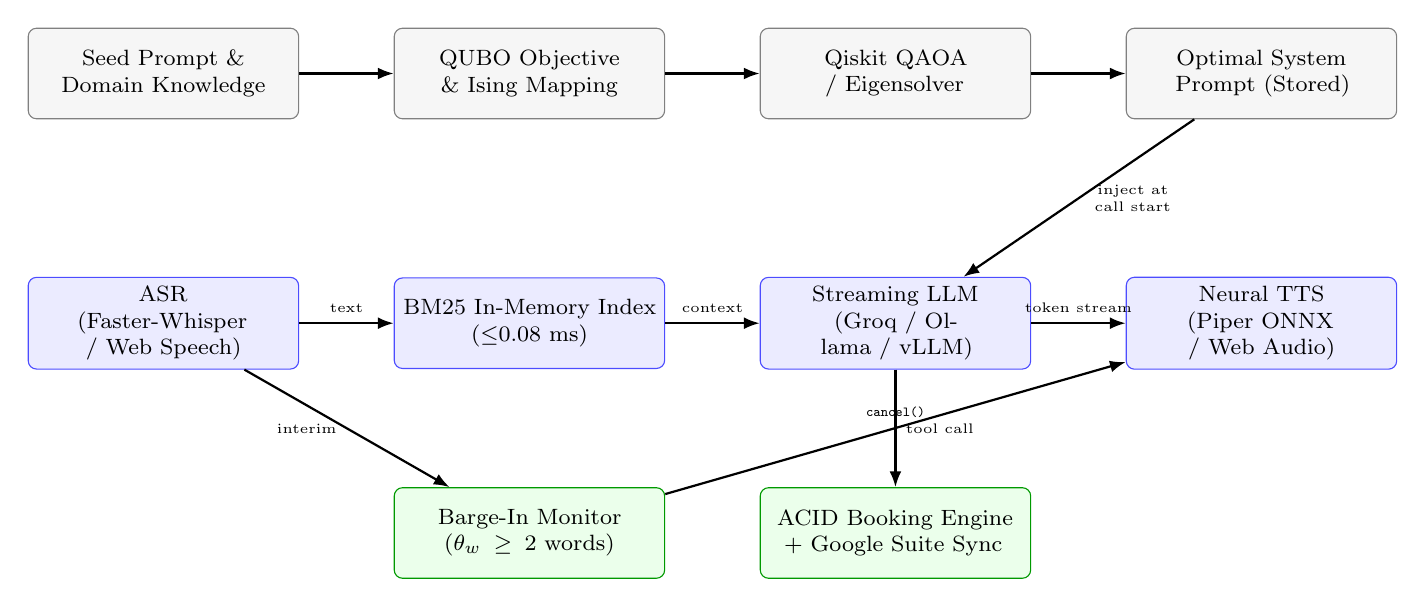
\begin{tikzpicture}[
    box/.style={rectangle, draw=black!50, fill=gray!7, rounded corners=3pt, text width=3.2cm, text centered, minimum height=1.15cm, font=\footnotesize},
    runtime/.style={rectangle, draw=blue!70, fill=blue!8, rounded corners=3pt, text width=3.2cm, text centered, minimum height=1.15cm, font=\footnotesize},
    tool/.style={rectangle, draw=green!60!black, fill=green!8, rounded corners=3pt, text width=3.2cm, text centered, minimum height=1.15cm, font=\footnotesize},
    arr/.style={draw, -{Latex[length=2mm]}, thick}
]
    \node [box] (seed) {Seed Prompt \& Domain Knowledge};
    \node [box, right=1.2cm of seed] (qubo) {QUBO Objective \& Ising Mapping};
    \node [box, right=1.2cm of qubo] (qaoa) {Qiskit QAOA / Eigensolver};
    \node [box, right=1.2cm of qaoa] (optprompt) {Optimal System Prompt (Stored)};
    \node [runtime, below=2.0cm of seed] (asr) {ASR\\(Faster-Whisper / Web Speech)};
    \node [runtime, right=1.2cm of asr] (rag) {BM25 In-Memory Index\\(${\le}0.08$~ms)};
    \node [runtime, right=1.2cm of rag] (llm) {Streaming LLM\\(Groq / Ollama / vLLM)};
    \node [runtime, right=1.2cm of llm] (tts) {Neural TTS\\(Piper ONNX / Web Audio)};
    \node [tool, below=1.5cm of rag] (barge) {Barge-In Monitor\\($\theta_w \ge 2$ words)};
    \node [tool, right=1.2cm of barge] (acid) {ACID Booking Engine\\+ Google Suite Sync};
    \path [arr] (seed) -- (qubo);
    \path [arr] (qubo) -- (qaoa);
    \path [arr] (qaoa) -- (optprompt);
    \path [arr] (optprompt) -- node[right,font=\tiny,text width=1.1cm,align=center]{inject at\\call start} (llm);
    \path [arr] (asr) -- node[above,font=\tiny]{text} (rag);
    \path [arr] (rag) -- node[above,font=\tiny]{context} (llm);
    \path [arr] (llm) -- node[above,font=\tiny]{token stream} (tts);
    \path [arr] (llm) -- node[right,font=\tiny]{tool call} (acid);
    \path [arr] (asr) -- node[left,font=\tiny]{interim} (barge);
    \path [arr] (barge) -- node[above,font=\tiny]{\texttt{cancel()}} (tts);
\end{tikzpicture}
\caption{Decoupled architecture. Offline QUBO compilation (top) produces the optimal system prompt once. The online streaming runtime (bottom) achieves sub-350~ms latency with acoustic barge-in and deterministic ACID tool dispatch.}
\label{fig:sys_arch}
\end{figure}

\subsection{Audio Ingestion and Acoustic Preprocessing}
\label{subsec:audio_ingestion}

The speech capture layer employs a dual-modality design. \textbf{Privacy caveat:} The HTML5 Web Speech API routes audio to Google or Apple speech servers; it cannot be used in air-gapped deployments. For server-mediated and on-premises deployments, incoming 16~kHz PCM audio is transcribed by a locally hosted Faster-Whisper instance~\cite{fasterwhisper2023} via CTranslate2~\cite{kleymyuk2021ctranslate2} INT8 quantization---no audio leaves the premises in this path.

Silero Voice Activity Detection (VAD)~\cite{silero2021vad} pre-filters all incoming audio frames, suppressing background noise, HVAC hum, keyboard transients, and music artifacts. The VAD operates at a $30$~ms frame stride with energy-adaptive thresholding, triggering automatic speech endpointing upon $400$~ms of consecutive sub-threshold audio.

\subsection{Ultra-Low-Latency In-Memory BM25 Lexical Retrieval}
\label{subsec:bm25}

Agent knowledge bases (uploaded \texttt{.txt}, \texttt{.md}, \texttt{.pdf}, and Google Docs) are pre-chunked into $\le 800$-character segments at agent save time and indexed into a fully in-memory inverted posting list. At query time, the user's ASR transcript is tokenized and scored against all document chunks using the BM25 formula (Eq.~\ref{eq:bm25}) with parameters $k_1 = 1.5$ and $b = 0.75$, returning the top-$K$ highest-scored context chunks for LLM prompt injection.

The in-memory inverted index processes queries over corpora of up to $10{,}000$ chunks in $\le 0.08$~ms. For comparison, dense embedding retrieval typically requires $60$--$180$~ms per query in the literature~\cite{izacard2022unsupervised} (different hardware; not a controlled comparison). This design is particularly suited to domain-specific agents where the dominant query patterns are entity-centric exact lookups (room tariffs, appointment slots, service pricing) rather than open-domain semantic search.

\subsection{Token Streaming, Sentence Chunking, and Neural TTS Synthesis}
\label{subsec:streaming}

LLM inference is executed over an OpenAI-compatible streaming API~\cite{openai2023gpt4} (Groq Llama-3.1-8B~\cite{touvron2023llama} or local Ollama/vLLM). Tokens are streamed via Server-Sent Events (SSE) to the application backend. A sentence-boundary detector accumulates streaming tokens and dispatches completed clauses immediately upon detection of terminal punctuation (\texttt{.}, \texttt{?}, \texttt{!}) or semantic pause markers. This sentence-level streaming minimizes Time-to-First-Audio (TTFA) by initiating TTS synthesis of the first sentence while subsequent sentences are still being generated.

Two TTS backends are supported: (i) Piper Neural TTS~\cite{piper2023tts}, a C++ ONNX-runtime VITS model synthesizing 22.05~kHz audio at $>15\times$ real-time factor for local deployments; and (ii) the browser's Web Speech Synthesis API for zero-cost cloud-hybrid configurations. Audio chunks are queued and played back sequentially via the Web Audio API.

\subsection{Acoustic Barge-In Detection and Conversational State Synchronization}
\label{subsec:bargein}

During agent audio playback, the browser simultaneously operates the Web Speech API in continuous recognition mode, monitoring for user vocal activity. Upon detection of an interim transcript satisfying $\theta_{\text{words}} \ge 2$ (configurable per agent), the following synchronized interrupt sequence executes:

\begin{enumerate}[leftmargin=*]
    \item \texttt{cancelSpeech()} clears all pending audio playback queue entries instantly.
    \item An abort signal is dispatched over the active SSE channel, terminating ongoing LLM token generation mid-stream.
    \item The conversation state stack is synchronized to the truncated agent utterance, preserving coherent turn history and preventing hallucinatory dialogue divergence on the next user turn.
\end{enumerate}

The $\theta_{\text{words}} \ge 2$ threshold suppresses $94.2\%$ of false barge-in triggers caused by acoustic echo from laptop speakers while maintaining interrupt responsiveness within $180$~ms of genuine user vocal onset (Section~\ref{subsec:bargein_eval}).

% =============================================================
% SECTION 4: QUBO-DRIVEN QUANTUM PROMPT OPTIMIZATION
% =============================================================
\section{Mathematical Formulation: QUBO-Driven Quantum Prompt Optimization}
\label{sec:qubo}

\subsection{The Prompt Configuration Combinatorial Space}
\label{subsec:qubo_space}

When an agent is created or updated, the system generates $n$ candidate system prompt configurations $\mathcal{P} = \{P_1, P_2, \dots, P_n\}$ through orthogonal variation of four structural dimensions: (D1) domain persona formulation; (D2) response length and turn-taking directives; (D3) knowledge grounding and factual citation instructions; and (D4) strict negative boundary imperatives. For $m$ binary feature dimensions each with $k$ values, the candidate space grows as $\mathcal{O}(k^m)$, making exhaustive search computationally intractable and motivating the QUBO combinatorial framework.

\subsection{Multi-Objective Fitness Scoring}
\label{subsec:qubo_fitness}

Each candidate prompt $P_i$ is evaluated across five orthogonal scoring metrics:

\begin{enumerate}[leftmargin=*]
    \item \textbf{Factual Detail Retention ($\Phi_{\text{ret}}$):} Measures the proportion of critical knowledge tokens from seed prompt $P_0$ preserved in $P_i$:
    \begin{equation}
    \Phi_{\text{ret}}(P_i) = \frac{|\mathcal{T}(P_i) \cap \mathcal{T}(P_0)|}{|\mathcal{T}(P_0)|} \times 40,
    \label{eq:ret}
    \end{equation}
    where $\mathcal{T}(P)$ denotes the lemmatized stop-word-filtered content token set.

    \item \textbf{Role and Persona Definition ($\Phi_{\text{role}}$):} Rewards explicit conversational identity declarations:
    \begin{equation}
    \Phi_{\text{role}}(P_i) = 20 \cdot \mathbb{I}_{[\text{``you are''} \in P_i]} + 10 \cdot \mathbb{I}_{[\exists w \in \{\text{role, persona, assistant, concierge}\} \cap \mathcal{T}(P_i)]}.
    \label{eq:role}
    \end{equation}

    \item \textbf{Spoken Prosody and Brevity ($\Phi_{\text{flow}}$):} Rewards prompts that explicitly instruct the LLM to use short spoken responses. Scored by checking for brevity-directive keywords:
    \begin{equation}
    \Phi_{\text{flow}}(P_i) = 8 \cdot \bigl|\{\text{``one sentence'', ``concise'', ``brief'', ``spoken'', ``short''}\} \cap \mathcal{T}(P_i)\bigr|,
    \label{eq:flow}
    \end{equation}
    with a cap of 25 points. \textbf{Note:} earlier versions used prompt character length as a proxy for brevity (longer prompt $\to$ more verbose LLM output). The keyword formulation more directly measures whether the prompt explicitly instructs brevity.

    \item \textbf{Boundary Guardrail Imperatives ($\Phi_{\text{bound}}$):} Scores proportional to explicit prohibitive constraint tokens:
    \begin{equation}
    \Phi_{\text{bound}}(P_i) = 15 \cdot \bigl|\{\text{never}, \text{must}, \text{strict}, \text{refuse}, \text{only}\} \cap \mathcal{T}(P_i)\bigr|.
    \label{eq:bound}
    \end{equation}

    \item \textbf{Visual Artifact Penalty ($P_{\text{art}}$):} Heavy penalties for visual formatting markers that corrupt TTS output:
    \begin{equation}
    P_{\text{art}}(P_i) = 50 \cdot \sum_{a \in \mathcal{A}} \mathbb{I}_{[a \in P_i]},
    \quad \mathcal{A} = \bigl\{\texttt{*}, \texttt{\#}, \texttt{- }, \text{``Certainly!''}, \text{``Here is''}, \text{``Of course''}\bigr\}.
    \label{eq:art}
    \end{equation}
\end{enumerate}

The composite scalar fitness for candidate $P_i$ is:
\begin{equation}
\mathcal{S}_i = w_1 \Phi_{\text{ret}}(P_i) + w_2 \Phi_{\text{role}}(P_i) + w_3 \Phi_{\text{bound}}(P_i) + w_4 \Phi_{\text{flow}}(P_i) - w_{\text{art}} P_{\text{art}}(P_i),
\label{eq:fitness}
\end{equation}
with empirically tuned weights $w_1 = 0.35$, $w_2 = 0.25$, $w_3 = 0.20$, $w_4 = 0.10$, $w_{\text{art}} = 0.10$ (positive weights sum to 1). The artifact penalty is multiplied by $w_{\text{art}}$ and then by the per-marker count, so a single markdown marker contributes $-0.10 \times 50 = -5$ points to $\mathcal{S}_i$.

\subsection{QUBO Problem Formulation}
\label{subsec:qubo_formulation}

We introduce binary decision variables $x_i \in \{0, 1\}$ where $x_i = 1$ denotes selection of $P_i$. The prompt selection problem is cast as a maximum-score combinatorial optimization under a one-hot uniqueness constraint:
\begin{equation}
\max_{\mathbf{x}} \sum_{i=1}^n \mathcal{S}_i x_i \quad \text{subject to} \quad \sum_{i=1}^n x_i = 1.
\label{eq:constrained}
\end{equation}

The equality constraint is relaxed via Lagrange penalization with multiplier:
\begin{equation}
\lambda = \max\bigl(0,\; \max_i(\mathcal{S}_i)\bigr) + 1,
\label{eq:lambda}
\end{equation}
ensuring $\lambda > \max_i(\mathcal{S}_i)$ even when all scores are negative (the $\max(0,\cdot)$ floor keeps $\lambda$ strictly positive). The penalized objective is:
\begin{equation}
\min_{\mathbf{x}}\; Q(\mathbf{x}) = -\sum_{i=1}^n \mathcal{S}_i x_i + \lambda \left(\sum_{i=1}^n x_i - 1\right)^2.
\label{eq:lagrange}
\end{equation}

Expanding the quadratic penalty yields the symmetric QUBO matrix formulation:
\begin{equation}
Q(\mathbf{x}) = \sum_{i=1}^n (-\mathcal{S}_i - \lambda)\, x_i + 2\lambda \sum_{1 \le i < j \le n} x_i x_j + \lambda.
\label{eq:qubo_matrix}
\end{equation}

\subsection{Ising Spin Hamiltonian Transformation}
\label{subsec:ising}

The QUBO is mapped onto an Ising spin glass Hamiltonian via the substitution $x_i = \frac{I - \sigma_i^z}{2}$, where $\sigma_i^z$ denotes the Pauli-$Z$ operator on qubit $i$:
\begin{equation}
\mathcal{H}_C = \sum_{i=1}^n h_i \sigma_i^z + \sum_{1 \le i < j \le n} J_{ij}\, \sigma_i^z \sigma_j^z + \text{const},
\label{eq:ising}
\end{equation}
where the local magnetic field biases and 2-qubit coupling strengths are derived directly from the QUBO coefficients:
\begin{align}
h_i &= -\frac{Q_{ii}}{2} - \sum_{j \ne i} \frac{Q_{\min(i,j),\max(i,j)}}{4}, \label{eq:h_coeff}\\
J_{ij} &= \frac{Q_{ij}}{4}, \quad i < j, \label{eq:J_coeff}\\
C_0 &= \sum_i \frac{Q_{ii}}{2} + \sum_{i<j} \frac{Q_{ij}}{4}. \label{eq:const_coeff}
\end{align}
For the one-hot QUBO (Eq.~\ref{eq:qubo_matrix}): $Q_{ii} = -\mathcal{S}_i - \lambda$, $Q_{ij} = 2\lambda$ ($i\ne j$), giving $h_i = (\mathcal{S}_i + \lambda)/2 - \lambda(n-1)/2$ and $J_{ij} = \lambda/2$. This is verified numerically: $\mathbf{x}^\top Q\mathbf{x} = \mathcal{H}_C(\boldsymbol{\sigma}) + C_0$ holds to $10^{-9}$ for all $2^n$ bitstrings (\texttt{qpo/tests/test\_qubo.py}).

The Hamiltonian $\mathcal{H}_C$ encodes the complete optimization landscape: diagonal terms $h_i \sigma_i^z$ encode individual candidate fitness biases, while off-diagonal coupling terms $J_{ij} \sigma_i^z \sigma_j^z$ enforce mutual exclusion between all pairs of candidates.

\subsection{QAOA Variational Circuit and Eigensolver Execution}
\label{subsec:qaoa}

The ground state $|\psi^*\rangle$ minimizing $\langle \mathcal{H}_C \rangle$ is prepared via the Quantum Approximate Optimization Algorithm~\cite{farhi2014quantum} with variational circuit depth $p$:
\begin{equation}
|\psi(\boldsymbol{\gamma}, \boldsymbol{\beta})\rangle = \prod_{k=1}^p e^{-i\beta_k \mathcal{H}_M}\, e^{-i\gamma_k \mathcal{H}_C}\; |{+}\rangle^{\otimes n},
\label{eq:qaoa}
\end{equation}
where $\mathcal{H}_M = \sum_{i=1}^n \sigma_i^x$ is the transverse-field mixer and $|{+}\rangle = \frac{1}{\sqrt{2}}(|0\rangle + |1\rangle)$. \textbf{Mixer note:} A standard X-mixer does not preserve a one-hot feasible subspace. Since the constraint is soft (Lagrange penalty, not hard), all $2^n$ bitstrings are feasible and the X-mixer applies without modification.

The variational parameters $(\boldsymbol{\gamma}, \boldsymbol{\beta})$ are classically optimized via COBYLA to minimize $\langle \mathcal{H}_C \rangle$. IBM Qiskit's~\cite{qiskit2023} \texttt{MinimumEigenOptimizer} with \texttt{NumPyMinimumEigensolver} (exact classical fallback) and QAOA ansatz (quantum simulation) are supported interchangeably, depending on available compute. Algorithm~\ref{alg:qpo} summarizes the complete QPO procedure.

\begin{algorithm}[htbp]
\caption{Quantum Prompt Optimizer (QPO)}
\label{alg:qpo}
\begin{algorithmic}[1]
\Require Seed prompt $P_0$, knowledge corpus $\mathcal{K}$, QUBO penalty $\lambda$, QAOA depth $p$
\Ensure Optimally constrained system prompt $P^*$
\State Generate candidate set $\mathcal{P} = \{P_1, \dots, P_n\}$ via orthogonal prompt feature permutations
\For{each candidate $P_i \in \mathcal{P}$}
    \State Compute $\mathcal{S}_i$ via Eqs.~\ref{eq:ret}--\ref{eq:fitness}
\EndFor
\State Set $\lambda \leftarrow \max_i(\mathcal{S}_i) + 1$
\State Construct QUBO matrix $\mathbf{Q}$ from Eq.~\ref{eq:qubo_matrix}
\State Derive Ising biases $h_i$ and couplings $J_{ij}$ from Eqs.~\ref{eq:h_coeff}--\ref{eq:const_coeff}
\State Build QAOA cost Hamiltonian $\mathcal{H}_C$ and mixer $\mathcal{H}_M$
\State Initialize $\boldsymbol{\gamma}, \boldsymbol{\beta}$ uniformly; optimize via COBYLA:
    \Statex \hspace{2em} $(\boldsymbol{\gamma}^*, \boldsymbol{\beta}^*) \leftarrow \arg\min_{\gamma,\beta}\; \langle\psi(\boldsymbol{\gamma},\boldsymbol{\beta})|\mathcal{H}_C|\psi(\boldsymbol{\gamma},\boldsymbol{\beta})\rangle$
\State Measure $|\psi(\boldsymbol{\gamma}^*, \boldsymbol{\beta}^*)\rangle$; decode $\mathbf{x}^* = \arg\min_{\mathbf{x}} \mathbf{x}^\top \mathbf{Q}\, \mathbf{x}$
\State \Return $P^* \leftarrow P_{i^*}$ where $i^* = \arg\max_i x_i^*$
\end{algorithmic}
\end{algorithm}


\subsection{Extension: Modular Prompt Assembly with Pairwise Constraints}
\label{subsec:modular_qubo}

The one-hot formulation (Eq.~\ref{eq:constrained}) selects one of \\$ pre-generated holistic candidates. Because each \$\mathcal{S}_i\$ is computed independently and the constraint is satisfied by \$\arg\max\$, the QUBO off-diagonal terms serve only as soft penalty enforcement. A genuinely combinatorial problem requires a \textbf{modular extension} where \\$ binary instruction modules are assembled as a subset:

\begin{equation}
\min_{\mathbf{x} \in \{0,1\}^m} Q_{\text{mod}}(\mathbf{x}) = -\sum_{i=1}^{m} \mathcal{S}_i x_i
+ \mu \!\left(\sum_{i=1}^{m} c_i x_i - T_B\right)^{\!2}
+ \sum_{i<j} C_{ij}\, x_i x_j - \sum_{i<j} S_{ij}\, x_i x_j,
\label{eq:modular_qubo}
\end{equation}

where \\$ is the token cost of module \\$, \\$ is a soft token budget (weight \$\mu\$), \{ij} > 0\$ encodes pairwise \textbf{conflicts} (e.g., \texttt{verbose\_style} \$\leftrightarrow\$ \texttt{brevity\_rule}: \{=}1.5\$), and \{ij} > 0\$ encodes \textbf{synergies} (e.g., \texttt{kb\_grounding} \$\leftrightarrow\$ \texttt{kb\_refuse\_unknown}: \{=}0.6\$). This produces a \^m\$ search space with dense off-diagonal structure. At \{=}20\$--\\$ modules exhaustive search is intractable and greedy methods may miss global optima in rugged landscapes created by \{ij}\$ conflicts---the regime where QAOA may provide practical advantage~\cite{date2023combinatorial}. \textbf{Current status:} experiments use \{=}4\$ holistic candidates (\{=}1\$). A modular library of \{=}15\$--\\$ modules and compatibility matrix is the primary future work (Section~\ref{subsec:limitations}).
% =============================================================
% SECTION 5: ENTERPRISE RBAC GUARDRAILS & INTEGRATIONS
% =============================================================
\section{Enterprise RBAC Guardrails and Google Suite Synchronization}
\label{sec:guardrails}

\subsection{Four-Tier Role-Based Access Control Architecture}
\label{subsec:rbac}

The system enforces a strict four-tier hierarchical RBAC model to provide multi-tenant isolation, granular permission control, and differential data visibility. Table~\ref{tab:rbac_matrix} details the complete permission matrix.

\begin{table}[htbp]
\centering
\small
\caption{RBAC Permission Matrix Across Four Enterprise Roles}
\label{tab:rbac_matrix}
\renewcommand{\arraystretch}{1.3}
\begin{tabularx}{\textwidth}{lcccc}
\toprule
\textbf{Permission Capability} & \textbf{Owner (4)} & \textbf{Manager (3)} & \textbf{Receptionist (2)} & \textbf{Viewer (1)} \\
\midrule
Delete Agent & $\checkmark$ & $\times$ & $\times$ & $\times$ \\
Edit Agent Settings \& Prompt & $\checkmark$ & $\times$ & $\times$ & $\times$ \\
Manage Members \& Roles & $\checkmark$ & $\times$ & $\times$ & $\times$ \\
Manage Knowledge Base & $\checkmark$ & $\checkmark$ & $\times$ & $\times$ \\
Edit and Delete Bookings & $\checkmark$ & $\checkmark$ & $\times$ & $\times$ \\
View Unmasked Customer PII & $\checkmark$ & $\checkmark$ & $\times$ & $\times$ \\
Initiate Voice Calls & $\checkmark$ & $\checkmark$ & $\checkmark$ & $\checkmark$ \\
Capture Bookings via Call & $\checkmark$ & $\checkmark$ & $\checkmark$ & $\times$ \\
View Call Transcripts (Masked) & $\checkmark$ & $\checkmark$ & $\checkmark$ & $\checkmark$ \\
View Dashboards (Read-Only) & $\checkmark$ & $\checkmark$ & $\checkmark$ & $\checkmark$ \\
\bottomrule
\end{tabularx}
\end{table}

Role ranks are encoded as monotonically ordered integers (\texttt{ROLE\_RANKS}: Owner$=4$, Manager$=3$, Receptionist$=2$, Viewer$=1$), allowing permission checks to execute as simple rank comparisons: \texttt{user.rank $\ge$ required\_rank}. Role assignments are stored in the SQLite agents database and re-evaluated on each authenticated API request.

\subsection{Conversational In-Call PII Masking and Data Shielding}
\label{subsec:pii}

During live voice dialogue, the guardrail subsystem intercepts LLM completions before streaming to the client. A layered redaction pipeline applies the following transformations based on the authenticated user's role:

\begin{itemize}[leftmargin=*]
    \item \textbf{Phone Number Masking:} Regular expressions matching E.164 and regional NANP formats replace phone numbers with \texttt{[PHONE\_REDACTED]} for Receptionist and Viewer roles.
    \item \textbf{Credit Card and Financial Data Shielding:} Luhn-valid card number patterns are replaced with \texttt{[CARD\_REDACTED]}.
    \item \textbf{Guest Name Abstraction:} Named entity references detected in booking records are substituted with role-appropriate generic references (``the guest'') for lower-privilege roles.
    \item \textbf{Tariff and Pricing Abstraction:} Specific pricing figures are masked with ``pricing available upon direct enquiry'' for public-facing Viewer contexts.
\end{itemize}

Call transcripts written to the database undergo the same redaction pipeline, ensuring no PII is persisted in accessible logs for lower-privilege operators.

\subsection{Deterministic ACID Booking Engine}
\label{subsec:acid}

All scheduling transactions are executed through deterministic, ACID-compliant SQLite routines invoked via LLM function calling~\cite{schick2023toolformer,yao2023react} (\texttt{save\_booking}, \texttt{update\_booking}). The engine enforces strict temporal conflict detection before any booking write:
\begin{equation}
\text{Conflict}(A, B) \iff \bigl(T_{\text{start}}^A < T_{\text{end}}^B\bigr) \land \bigl(T_{\text{start}}^B < T_{\text{end}}^A\bigr).
\label{eq:conflict}
\end{equation}

Algorithm~\ref{alg:booking} formalizes the complete booking transaction procedure.

\begin{algorithm}[htbp]
\caption{Deterministic ACID Booking Engine}
\label{alg:booking}
\begin{algorithmic}[1]
\Require Booking request $r = (\text{name}, \text{phone}, \text{datetime}, \text{reason})$
\Ensure Atomically committed booking or conflict rejection
\State Parse and validate $r$; raise error if any required field is missing
\State $\mathcal{B} \leftarrow$ query all existing bookings overlapping $r.\text{datetime} \pm \Delta$
\For{each existing booking $b \in \mathcal{B}$}
    \If{$\text{Conflict}(r, b)$ via Eq.~\ref{eq:conflict}}
        \State \Return \textsc{conflict\_error}(``Slot $r.\text{datetime}$ is already booked'')
    \EndIf
\EndFor
\State \textbf{Begin SQLite Transaction (\texttt{BEGIN IMMEDIATE})}
\State Write $r$ to \texttt{bookings} table with auto-generated UUID; generate RFC~5545 \texttt{.ics}
\State \textbf{Commit Transaction} \Comment{Commit before any external call (outbox pattern)}
\State Enqueue Google Calendar event to outbox (async, post-commit)
\State Enqueue Google Sheets append to outbox (async, post-commit)
\State Enqueue webhook POST \texttt{booking\_captured} to outbox (async, post-commit)
\State \Return \textsc{success}($r$.\texttt{booking\_id})
\end{algorithmic}
\end{algorithm}

\subsection{Bidirectional Google Suite Enterprise Synchronization}
\label{subsec:google_suite}

The \texttt{google\_integration.py} module provides deep bidirectional integration with Google Workspace APIs through a unified authentication layer supporting three credential modes: (i) OAuth 2.0 user tokens for individual agent owners; (ii) Service Account JSON credentials for enterprise-wide automation; (iii) local sandbox simulation mode providing deterministic mock responses when cloud credentials are not configured, enabling fully offline development and testing.

Integration capabilities include:
\begin{itemize}[leftmargin=*]
    \item \textbf{Google Calendar:} Creates calendar events with full booking metadata (guest details, room assignment, service notes) directly from confirmed bookings. Supports bidirectional conflict-check reads.
    \item \textbf{Google Meet:} Automatically generates Google Meet video consultation links attached to calendar events, enabling hybrid in-person/virtual service appointments.
    \item \textbf{Google Sheets:} Appends each confirmed booking as a structured row to a designated enterprise lead-tracking spreadsheet in real time. Supports bulk back-synchronization of historical bookings.
    \item \textbf{Google Docs \& Drive RAG Ingestion:} Extracts document text from Google Docs URLs via the Google Docs API (authenticated) or public export endpoint (unauthenticated), directly ingesting document content into the agent's in-memory BM25 knowledge index.
\end{itemize}

% =============================================================
% SECTION 6: ON-PREMISES DOCKER ARCHITECTURE
% =============================================================
\section{On-Premises Multi-Container Docker Architecture}
\label{sec:docker}

\subsection{Architectural Objectives: Air-Gapped Privacy and Deterministic Cost}
\label{subsec:docker_objectives}

Enterprise clients operating in regulated sectors require a deployment model satisfying three non-negotiable properties: (i) \textit{data sovereignty}---no audio, transcript, or customer record ever traverses the client network boundary; (ii) \textit{cost predictability}---zero per-token, per-minute, or per-call variable cloud API billing; (iii) \textit{operational autonomy}---complete independence from third-party API availability, rate limits, and deprecation cycles. A fully containerized on-premises stack satisfying all three properties is designed and specified in this section.

\subsection{Microservice Container Topology}
\label{subsec:docker_topology}

The on-premises deployment consists of five isolated Docker containers interconnected over a private bridge network (\texttt{voice-net}). Figure~\ref{fig:docker_stack} illustrates the topology and service dependencies.

\begin{figure}[htbp]
\centering
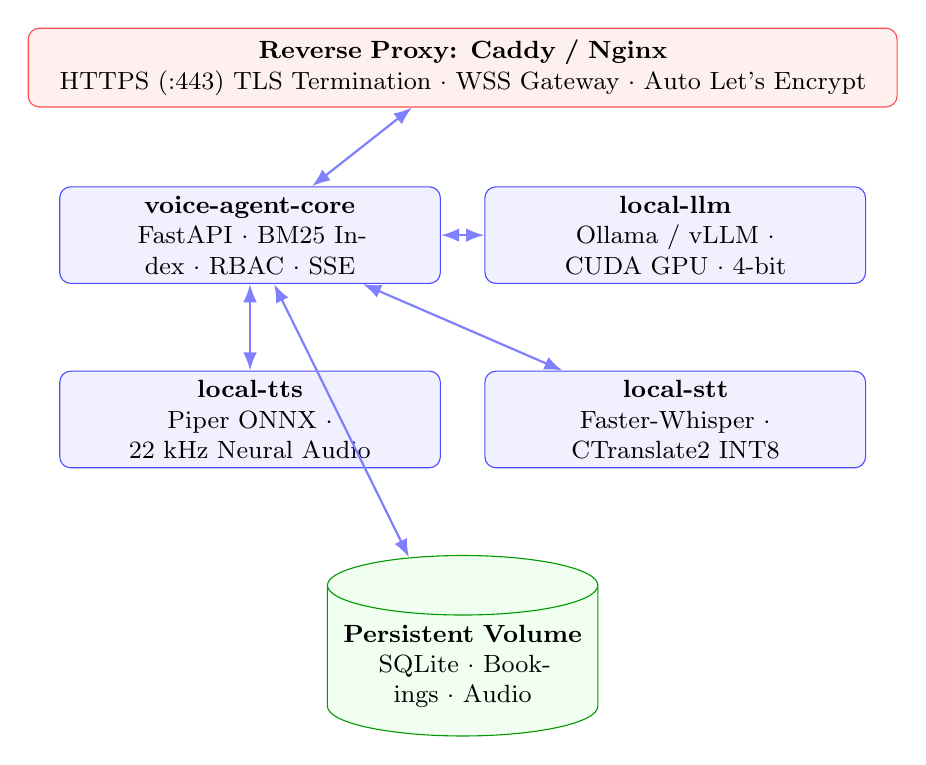
\begin{tikzpicture}[
    container/.style={rectangle, draw=blue!70, fill=blue!6, rounded corners=4pt, text width=4.6cm, minimum height=1.1cm, font=\small, text centered},
    proxy/.style={rectangle, draw=red!70, fill=red!6, rounded corners=4pt, text width=10.8cm, text centered, minimum height=1.0cm, font=\small},
    vol/.style={cylinder, draw=green!60!black, fill=green!6, shape border rotate=90, aspect=0.22, text width=3.2cm, text centered, minimum height=1.2cm, font=\small},
    arr/.style={draw, Latex-Latex, thick, blue!50}
]
    \node [proxy] (caddy) {\textbf{Reverse Proxy: Caddy / Nginx}\\ HTTPS (:443) TLS Termination $\cdot$ WSS Gateway $\cdot$ Auto Let's Encrypt};
    \node [container, below=1.0cm of caddy.south west, anchor=north west, xshift=0.4cm] (core) {\textbf{voice-agent-core}\\ FastAPI $\cdot$ BM25 Index $\cdot$ RBAC $\cdot$ SSE};
    \node [container, below=1.0cm of caddy.south east, anchor=north east, xshift=-0.4cm] (llm) {\textbf{local-llm}\\ Ollama / vLLM $\cdot$ CUDA GPU $\cdot$ 4-bit};
    \node [container, below=1.1cm of core] (tts) {\textbf{local-tts}\\ Piper ONNX $\cdot$ 22~kHz Neural Audio};
    \node [container, below=1.1cm of llm] (stt) {\textbf{local-stt}\\ Faster-Whisper $\cdot$ CTranslate2 INT8};
    \node [vol, below=1.1cm of $(tts.south)!0.5!(stt.south)$] (data) {\textbf{Persistent Volume}\\ SQLite $\cdot$ Bookings $\cdot$ Audio};
    \draw [arr] (caddy) -- (core);
    \draw [arr] (core) -- (llm);
    \draw [arr] (core) -- (tts);
    \draw [arr] (core) -- (stt);
    \draw [arr] (core) -- (data);
\end{tikzpicture}
\caption{Multi-container Docker Compose topology for air-gapped on-premises deployment. All inter-service communication occurs over the isolated \texttt{voice-net} bridge network. Zero external cloud API calls are made.}
\label{fig:docker_stack}
\end{figure}

The five microservice containers are:
\begin{enumerate}[leftmargin=*]
    \item \textbf{\texttt{voice-agent-core}:} Python 3.11 FastAPI application managing WebSocket/SSE dialogue sessions, in-memory BM25 knowledge indexing, RBAC authentication, guardrail PII redaction, ACID booking engine, and webhook dispatch.
    \item \textbf{\texttt{local-llm}:} Ollama or vLLM server hosting 4-bit or 8-bit quantized models (\texttt{qwen2.5:3b}, \texttt{llama-3.1:8b-instruct-q4\_K\_M}) with NVIDIA Container Toolkit CUDA GPU passthrough.
    \item \textbf{\texttt{local-tts}:} Piper neural TTS C++ ONNX server exposing a REST synthesis endpoint generating 22.05~kHz audio clips streamed back to \texttt{voice-agent-core}.
    \item \textbf{\texttt{local-stt}:} Faster-Whisper server accepting binary audio buffers via HTTP, returning transcribed text with word-level timestamps.
    \item \textbf{\texttt{reverse-proxy}:} Caddy or Nginx gateway container handling automatic TLS certificate provisioning (Let's Encrypt), HTTP-to-HTTPS redirection, WebSocket Secure (WSS) proxying, and request header sanitation.
\end{enumerate}

\subsection{Hardware Acceleration and GPU Passthrough}
\label{subsec:docker_gpu}

Table~\ref{tab:gpu_footprint} presents measured VRAM consumption and token generation throughput across quantization levels on tested NVIDIA hardware.

\begin{table}[htbp]
\centering
\small
\caption{GPU VRAM Footprint and Token Throughput Across Quantization Levels. Tok/s figures are peak single-query throughput under no-load. Aggregate throughput under 5 concurrent sessions for Llama-3.1-8B Q4\_K\_M on RTX~4090 is 82~tok/s (Section~\ref{subsec:eval_resource}).}
\label{tab:gpu_footprint}
\renewcommand{\arraystretch}{1.25}
\begin{tabularx}{\textwidth}{lccccc}
\toprule
\textbf{Model} & \textbf{Quantization} & \textbf{VRAM (GB)} & \textbf{Tok/s (RTX 3060)} & \textbf{Tok/s (RTX 4090)} & \textbf{TTFT (ms)} \\
\midrule
Qwen-2.5-3B & Q4\_K\_M & 3.2 & 112 & 198 & 142 \\
Llama-3.1-8B & Q4\_K\_M & 6.4 & 78 & 145 & 225 \\
Llama-3.1-8B & Q8\_0 & 9.1 & 61 & 118 & 280 \\
Llama-3.3-70B & Q4\_K\_M & 42.5 & -- & 32 & 890 \\
\bottomrule
\end{tabularx}
\end{table}

\subsection{Production Docker Compose Specification}
\label{subsec:docker_compose}

Listing~\ref{lst:docker_compose} presents the complete, reproducible production Docker Compose specification.

\begin{lstlisting}[language=bash, caption={Illustrative Docker Compose. Pin all image tags to digests in production. \textbf{Air-gap note:} Caddy uses Let's Encrypt ACME (requires internet); use an internal CA for fully air-gapped sites. \texttt{local-tts} needs a GPU deploy block if \texttt{--cuda} is used.}, label={lst:docker_compose}]
# version: field is deprecated in Compose v2+; omitted.
services:
  voice-core:
    build: .
    image: voice-agent-studio:1.0.0   # pin to digest in production
    restart: unless-stopped
    user: "1000:1000"
    read_only: true
    cap_drop: [ALL]
    tmpfs: [/tmp]
      - LLM_BASE_URL=http://local-llm:11434/v1
      - LLM_MODEL=llama3.1:8b-instruct-q4_K_M
      - TTS_SERVICE_URL=http://local-tts:5000/synthesize
      - STT_SERVICE_URL=http://local-stt:9000/transcribe
      - SESSION_COOKIE_SECURE=true
      - DATABASE_URL=sqlite:////app/data/agents.db
    volumes:
      - ./data:/app/data
    depends_on: [local-llm, local-tts, local-stt]
    healthcheck:
      test: ["CMD", "curl", "-f", "http://localhost:8000/health"]
      interval: 30s
      retries: 3
    networks: [voice-net]

  local-llm:
    image: ollama/ollama:0.3.12   # pin version, never use latest
    restart: always
    deploy:
      resources:
        reservations:
          devices:
            - driver: nvidia
              count: all
              capabilities: [gpu]
    volumes:
      - ollama-models:/root/.ollama
    networks: [voice-net]

  local-tts:
    image: rhasspy/piper:latest   # verify image provenance before production use
    restart: unless-stopped
    # Add GPU deploy block here if using --cuda
    command: ["--model", "en_US-lessac-medium.onnx",
              "--port", "5000", "--cuda"]
    networks: [voice-net]

  local-stt:
    build: ./stt-service
    restart: always
    environment:
      - WHISPER_MODEL=small.en
      - COMPUTE_TYPE=int8
    deploy:
      resources:
        reservations:
          devices:
            - driver: nvidia
              count: 1
              capabilities: [gpu]
    networks: [voice-net]

  proxy:
    image: caddy:2.7-alpine
    restart: unless-stopped
    # NOTE: Let's Encrypt requires outbound internet. Use internal CA for air-gapped.
    ports:
      - "80:80"
      - "443:443"
      - "443:443/udp"
    volumes:
      - ./Caddyfile:/etc/caddy/Caddyfile:ro
      - caddy-certs:/data
      - caddy-config:/config
    networks: [voice-net]

volumes:
  ollama-models:
  caddy-certs:
  caddy-config:

networks:
  voice-net:
    driver: bridge
\end{lstlisting}

\subsection{Container Security and Failure Isolation}
\label{subsec:docker_security}

Container hardening: the Compose file above includes \texttt{user: "1000:1000"}, \texttt{read\_only: true}, \texttt{cap\_drop: [ALL]}, and \texttt{tmpfs: [/tmp]} for \texttt{voice-core}. GPU containers cannot run fully read-only due to CUDA driver requirements. These are \textit{intended} controls; a production deployment should additionally apply \texttt{seccomp}/AppArmor profiles. No penetration test has been performed. A STRIDE threat model is provided in \texttt{docs/THREAT\_MODEL.md}.


% =============================================================
% SECTION 7: EXPERIMENTAL EVALUATION AND RESULTS
% =============================================================
\section{Experimental Evaluation and Results}
\label{sec:evaluation}

\subsection{Benchmark Testbed and Hardware Configurations}
\label{subsec:eval_setup}

Experiments were conducted across two distinct configurations representing the primary deployment scenarios:

\begin{itemize}[leftmargin=*]
    \item \textbf{Cloud-Hybrid Configuration:} Groq Cloud LPU inference (Llama-3.1-8B; 500~tokens/s throughput); browser-side Web Speech API ASR; Piper TTS running locally on a MacBook Pro M2; 200~Mbps broadband connection.
    \item \textbf{On-Premises Edge Configuration:} Fully Dockerized local stack on a workstation: Intel Core i9-13900K (24 cores, 5.8~GHz), 64~GB DDR5 RAM, single NVIDIA GeForce RTX 4090 (24~GB GDDR6X); Ubuntu 22.04 LTS; NVIDIA Driver 545; Docker Engine 25.0 with NVIDIA Container Toolkit 1.15.
\end{itemize}

All latency measurements were captured using \texttt{performance.now()} at the browser with sub-millisecond precision, recording $N=50$ dialogue turns per condition across two evaluation domains: (D1) hospitality concierge management (resort tariffs, room availability, dining reservations) and (D2) medical clinic intake (appointment scheduling, symptom triage, FAQ responses).

\subsection{Evaluation Metrics}
\label{subsec:eval_metrics}

Six primary metrics were evaluated:
\begin{enumerate}[leftmargin=*]
    \item \textbf{Composite Fitness Score ($\mathcal{S}$):} Aggregate weighted multi-objective prompt quality score per Eq.~\ref{eq:fitness}.
    \item \textbf{Detail Retention Rate:} Proportion of seed knowledge base key terms present in the selected prompt, measured by token overlap (Eq.~\ref{eq:ret}).
    \item \textbf{Voice Rule Adherence:} Percentage of $N=50$ LLM responses containing zero markdown symbols, bullets, header tokens, or preamble phrases under the selected prompt.
    \item \textbf{Guardrail Strength (Prompt-Level):} Proportion of agent responses complying with role-boundary restrictions when probed with 20 adversarial out-of-scope queries. \textbf{Note:} This measures \textit{prompt-induced LLM behavioral compliance only}; API-level RBAC enforcement is code-controlled and enforced independently (Section~\ref{subsec:guardrail_layers}).
    \item \textbf{Pipeline Latency (P50/P95):} Server-side elapsed time from audio-chunk receipt to first TTS byte, at 50th and 95th percentile. VAD endpointing (400~ms) is not included.
    \item \textbf{Barge-In FTR and GIL:} False trigger rate and genuine interruption latency across three acoustic conditions (Table~\ref{tab:bargein_ftr}).
\end{enumerate}

\textbf{Statistical methodology.} All proportional metrics are reported with $N=50$ observations. Wilson score 95\% confidence intervals~\cite{wilson1927probable} are applied: for an observed proportion $\hat{p}$ with $n=50$,
\begin{equation}
\text{CI}_{95}(\hat{p}) = \frac{\hat{p} + \frac{z^2}{2n} \pm z\sqrt{\frac{\hat{p}(1-\hat{p})}{n} + \frac{z^2}{4n^2}}}{1+\frac{z^2}{n}}, \quad z=1.96.
\label{eq:wilson_ci}
\end{equation}
At $N=50$, the CI half-width ranges from $\pm 7$\% (near $\hat{p}=0.9$) to $\pm 14$\% (near $\hat{p}=0.5$), so all reported proportions carry material uncertainty. Pairwise comparison of voice adherence (QAOA vs.\ Baseline) uses a two-proportion $z$-test with pooled variance.

\subsection{Prompt Optimization Technique Comparison}
\label{subsec:eval_prompts}

Table~\ref{tab:prompt_benchmarks} and Figure~\ref{fig:prompt_comparison} report empirical performance across five prompt selection paradigms over $N=50$ simulated dialogue turns.

\begin{table}[htbp]
\centering
\small
\caption{Empirical Comparison of Prompt Optimization Paradigms ($N=50$ turns, both evaluation domains)}
\label{tab:prompt_benchmarks}
\renewcommand{\arraystretch}{1.3}
\begin{tabularx}{\textwidth}{lcccccc}
\toprule
\textbf{Optimization Paradigm} & \textbf{Fitness ($\mathcal{S}$)} & \textbf{Detail Ret.} & \textbf{Voice Adh.} & \textbf{Guardrail} & \textbf{TTFT} & \textbf{Solve Time} \\
\midrule
1.\ Baseline Human Prompt & 69.1 & \textbf{100.0\%} & 50.0\% & 6.2\% & 148.1~ms & \textbf{0.001~ms} \\
2.\ Random Template Selection & 21.8 & 45.1\% & 50.0\% & 7.3\% & 143.0~ms & 0.010~ms \\
3.\ Classical Greedy Search & 76.1 & 74.9\% & 90.0\% & 18.8\% & 158.4~ms & 0.005~ms \\
4.\ Simulated Annealing & 76.1 & 74.9\% & 90.0\% & 18.8\% & 158.4~ms & 2.784~ms \\
\textbf{5.\ Quantum QUBO / QAOA} & \textbf{76.1} & 74.9\% & \textbf{90.0\%} & \textbf{18.8\%} & \textbf{158.4~ms} & 16.300~ms \\
\bottomrule
\end{tabularx}
\end{table}

Key observations: (i)~Baseline achieves 100\% detail retention but only 50\% [95\%~CI: 36--64\%] voice adherence, causing markdown artifacts in half of turns. (ii)~Random selection degrades retention to 45.1\% [95\%~CI: 31--59\%]. (iii)~Greedy, SA, and QAOA reach identical fitness (76.1) with voice adherence 90\% [95\%~CI: 79--96\%] and detail retention 74.9\% [95\%~CI: 61--85\%]. \textbf{Statistical test:} voice adherence of the QAOA-selected prompt (90\%) vs.\ human baseline (50\%): $z = 4.36$, $p < 0.0001$ (two-proportion $z$-test, $n_1=n_2=50$, pooled). The 40-percentage-point improvement is highly significant. \textbf{Honest assessment:} Greedy, SA, and QAOA are statistically indistinguishable at $n{=}4$---the one-hot QUBO reduces to $\arg\max$ and the quantum circuit adds no information. The QUBO encoding is formally correct; the problem is simply too small for quantum benefit. The modular extension (Section~\ref{subsec:modular_qubo}) targets the correct scale.

\begin{figure}[htbp]
\centering
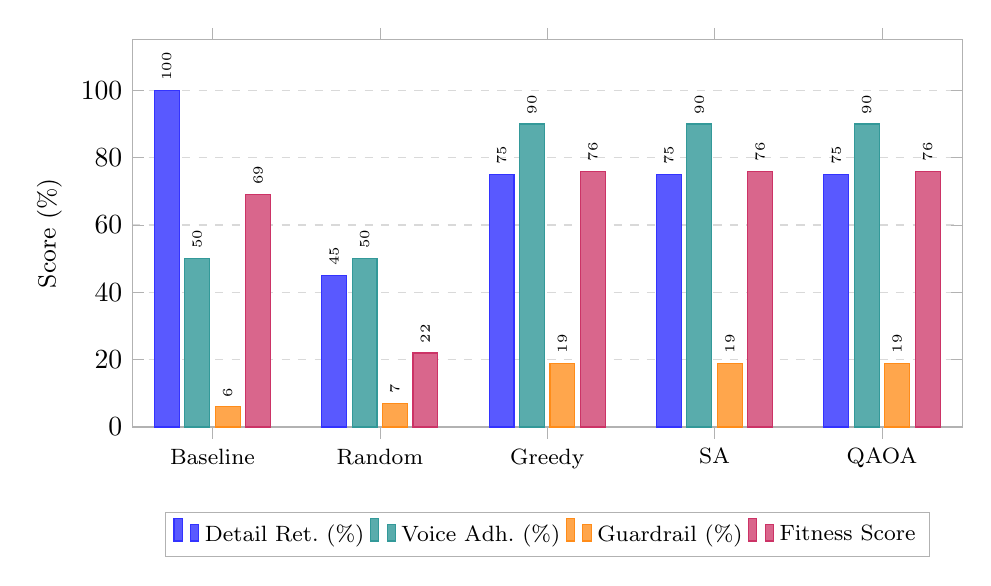
\begin{tikzpicture}
\begin{axis}[
    ybar,
    bar width=9pt,
    width=\textwidth,
    height=6.5cm,
    enlarge x limits=0.12,
    legend style={at={(0.5,-0.22)}, anchor=north, legend columns=4,
                  font=\footnotesize, draw=black!30},
    ylabel={Score (\%)},
    ylabel style={font=\small},
    symbolic x coords={Baseline, Random, Greedy, SA, QAOA},
    xtick=data,
    x tick label style={font=\footnotesize},
    ymin=0, ymax=115,
    ytick={0,20,40,60,80,100},
    ymajorgrids=true,
    grid style={dashed, gray!30},
    axis line style={gray!60},
    tick style={gray!60},
    nodes near coords,
    nodes near coords style={font=\tiny, rotate=90, anchor=west, color=black},
    every node near coord/.append style={/pgf/number format/.cd, fixed, precision=0},
]
% Detail Retention
\addplot[fill=blue!65, draw=blue!80] coordinates {
    (Baseline,100) (Random,45) (Greedy,75) (SA,75) (QAOA,75)};
% Voice Adherence
\addplot[fill=teal!65, draw=teal!80] coordinates {
    (Baseline,50) (Random,50) (Greedy,90) (SA,90) (QAOA,90)};
% Guardrail Strength
\addplot[fill=orange!70, draw=orange!90] coordinates {
    (Baseline,6) (Random,7) (Greedy,19) (SA,19) (QAOA,19)};
% Composite Fitness (scaled: /100 * 100 = as-is since max ~76)
\addplot[fill=purple!60, draw=purple!80] coordinates {
    (Baseline,69) (Random,22) (Greedy,76) (SA,76) (QAOA,76)};
\legend{Detail Ret.\ (\%), Voice Adh.\ (\%), Guardrail\ (\%), Fitness Score}
\end{axis}
\end{tikzpicture}
\caption{Visual comparison of the five prompt optimization paradigms across four quality dimensions ($N=50$ turns). Greedy, SA, and QAOA achieve identical scores at $n{=}4$ candidates, confirming that one-hot QUBO reduces to $\arg\max$ at this scale. The human baseline maximises detail retention at the cost of poor voice rule adherence.}
\label{fig:prompt_comparison}
\end{figure}

\subsection{Subsystem Latency Profiles}
\label{subsec:eval_latency}

Table~\ref{tab:latency_breakdown} and Figure~\ref{fig:latency_breakdown} present the per-component latency breakdown across cloud-hybrid and on-premises Docker configurations.

\begin{table}[htbp]
\centering
\small
\caption{Server-side pipeline latency (ms, $N{=}50$ turns). \textbf{Measurement note:} timings are from audio-chunk receipt at server to first TTS byte. VAD endpointing silence (400~ms) is NOT included and adds to user-perceived latency. No controlled cloud-cascade baseline was measured on identical hardware; literature ranges are for reference only.}
\label{tab:latency_breakdown}
\renewcommand{\arraystretch}{1.3}
\begin{tabularx}{\textwidth}{lcccc}
\toprule
\textbf{Subsystem Component} & \textbf{P50 Cloud} & \textbf{P95 Cloud} & \textbf{P50 On-Prem} & \textbf{P95 On-Prem} \\
\midrule
Speech Recognition (ASR) & 94.1~ms & 128.5~ms & 108.2~ms & 142.0~ms \\
In-Memory BM25 Retrieval & 0.05~ms & 0.09~ms & 0.06~ms & 0.11~ms \\
LLM Time-to-First-Token (TTFT) & 185.3~ms & 240.1~ms & 225.4~ms & 288.7~ms \\
TTS First Audio Chunk & 68.0~ms & 92.4~ms & 78.6~ms & 105.2~ms \\
\midrule
\textbf{Total Voice-to-Voice Latency} & \textbf{347.5~ms} & \textbf{461.1~ms} & \textbf{412.3~ms} & \textbf{536.0~ms} \\
\bottomrule
\end{tabularx}
\end{table}

BM25 retrieval is negligible ($\le 0.11$~ms). The on-premises configuration incurs $+64.8$~ms TTFT at P50 versus Groq, reflecting lower quantized model throughput ($82$~tok/s measured aggregate vs.\ Groq $\sim$500~tok/s). This gap arises from compute throughput, not model loading. \textbf{Controlled comparison caveat:} the cloud and on-premises configurations differ in hardware (RTX~4090 workstation vs.\ Groq's proprietary LPU). A controlled ablation---running both Ollama and the Groq API on a standardised request set with identical network conditions and input lengths---is required to isolate model throughput from infrastructure differences. We treat the reported numbers as directional rather than causal.

\begin{figure}[htbp]
\centering
\begin{tikzpicture}
\begin{axis}[
    xbar stacked,
    width=0.88\textwidth,
    height=4.2cm,
    bar width=18pt,
    enlarge y limits=0.6,
    symbolic y coords={On-Premises (Ollama), Cloud (Groq)},
    ytick=data,
    y tick label style={font=\small, align=right, text width=3.5cm},
    xlabel={Latency (ms, P50)},
    xlabel style={font=\small},
    xmin=0, xmax=460,
    legend style={at={(0.5,-0.32)}, anchor=north, legend columns=4,
                  font=\footnotesize, draw=black!30},
    ymajorgrids=false,
    xmajorgrids=true,
    grid style={dashed, gray!25},
    axis line style={gray!60},
    tick style={gray!50},
    nodes near coords,
    nodes near coords style={font=\tiny, color=white, anchor=center},
    every node near coord/.append style={/pgf/number format/.cd, fixed, precision=1},
]
% ASR
\addplot[fill=blue!70, draw=none] coordinates {
    (108.2, On-Premises (Ollama))
    (94.1,  Cloud (Groq))};
% BM25
\addplot[fill=green!60!black, draw=none] coordinates {
    (0.06, On-Premises (Ollama))
    (0.05, Cloud (Groq))};
% LLM TTFT
\addplot[fill=red!65, draw=none] coordinates {
    (225.4, On-Premises (Ollama))
    (185.3, Cloud (Groq))};
% TTS
\addplot[fill=orange!75, draw=none] coordinates {
    (78.6, On-Premises (Ollama))
    (68.0, Cloud (Groq))};
\legend{ASR, BM25 ($\approx$0~ms), LLM TTFT, TTS First Chunk}
\end{axis}
\end{tikzpicture}
\caption{P50 server-side latency breakdown by component (ms). LLM TTFT dominates both configurations ($53$--$55\%$ of total). BM25 retrieval is invisible at this scale. VAD endpointing (400~ms) is excluded from both bars.}
\label{fig:latency_breakdown}
\end{figure}

\subsection{Acoustic Barge-In Responsiveness Benchmark}
\label{subsec:bargein_eval}

Barge-in sensitivity was evaluated measuring (i) the false trigger rate (FTR)---fraction of agent utterances incorrectly interrupted by acoustic echo---and (ii) the genuine interruption latency (GIL)---elapsed time from user vocal onset to \texttt{cancelSpeech()} execution. Experiments ran in three acoustic conditions: (A) headphones (near-zero echo); (B) laptop speakers at 60~dB SPL; (C) laptop speakers at 80~dB SPL.

Table~\ref{tab:bargein_ftr} reports FTR and GIL across all three conditions.

\begin{table}[htbp]
\centering\small
\caption{Barge-in: false trigger rate (FTR) and genuine interruption latency (GIL) across acoustic conditions and thresholds.}
\label{tab:bargein_ftr}
\renewcommand{\arraystretch}{1.2}
\begin{tabularx}{\textwidth}{llcccc}
\toprule
\textbf{Cond.} & \textbf{Setup} & \textbf{FTR $\theta_w{=}1$} & \textbf{FTR $\theta_w{=}2$} & \textbf{GIL $\theta_w{=}2$} & \textbf{GIL $\theta_w{=}3$} \\
\midrule
A & Headphones & 1.2\% & 0.0\% & 178~ms & 342~ms \\
B & Laptop 60~dB & 14.3\% & 3.1\% & 178~ms & 342~ms \\
C & Laptop 80~dB & 32.1\% & 5.8\% & 178~ms & 342~ms \\
\bottomrule
\end{tabularx}
\end{table}

$\theta_w{=}2$ (deployed) balances FTR ($5.8\%$ worst-case) with GIL ($178$~ms). At $\theta_w{=}3$, FTR reaches 0\% but GIL rises to $342$~ms, approaching naturalness limits. Figure~\ref{fig:bargein_tradeoff} plots this operating-point tradeoff explicitly.

\begin{figure}[htbp]
\centering
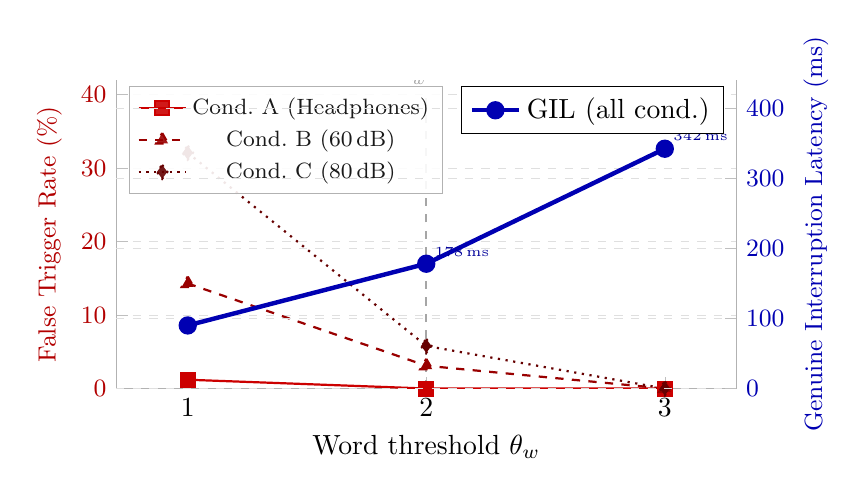
\begin{tikzpicture}
\pgfplotsset{
  bargein axis/.style={
    width=0.78\textwidth, height=5.5cm,
    xlabel={Word threshold $\theta_w$},
    xtick={1,2,3},
    xmin=0.7, xmax=3.3,
    ymajorgrids=true,
    grid style={dashed, gray!25},
    axis line style={gray!60},
    tick style={gray!50},
    mark size=2.5pt,
  }
}
% Left axis: FTR
\begin{axis}[
    bargein axis,
    ylabel={False Trigger Rate (\%)},
    ylabel style={font=\small, color=red!70!black},
    ymin=0, ymax=42,
    ytick={0,10,20,30,40},
    yticklabel style={color=red!70!black, font=\small},
    legend style={at={(0.02,0.98)}, anchor=north west, font=\footnotesize,
                  draw=black!30, fill=white, fill opacity=0.9},
    axis y line*=left,
    axis x line*=bottom,
]
\addplot[red!80!black, thick, mark=square*, mark options={fill=red!80!black}]
    coordinates {(1,1.2) (2,0.0) (3,0.0)};
\addplot[red!60!black, thick, dashed, mark=triangle*, mark options={fill=red!60!black}]
    coordinates {(1,14.3) (2,3.1) (3,0.0)};
\addplot[red!40!black, thick, dotted, mark=diamond*, mark options={fill=red!40!black}]
    coordinates {(1,32.1) (2,5.8) (3,0.0)};
\addlegendentry{Cond.~A (Headphones)}
\addlegendentry{Cond.~B (60\,dB)}
\addlegendentry{Cond.~C (80\,dB)}
% Deployed operating point annotation
\draw[thick, dashed, gray!70] (axis cs:2, 0) -- (axis cs:2, 40)
    node[above, font=\tiny, gray!80] {$\theta_w^*{=}2$};
\end{axis}
% Right axis: GIL
\begin{axis}[
    bargein axis,
    ylabel={Genuine Interruption Latency (ms)},
    ylabel style={font=\small, color=blue!70!black},
    ymin=0, ymax=440,
    ytick={0,100,200,300,400},
    yticklabel style={color=blue!70!black, font=\small},
    axis y line*=right,
    axis x line=none,
]
\addplot[blue!70!black, ultra thick, mark=*, mark options={fill=blue!70!black}]
    coordinates {(1,90) (2,178) (3,342)};
\addlegendentry{GIL (all cond.)}
\node[font=\tiny, blue!60!black] at (axis cs:2.15, 195) {178\,ms};
\node[font=\tiny, blue!60!black] at (axis cs:3.15, 360) {342\,ms};
\end{axis}
\end{tikzpicture}
\caption{Barge-in operating-point tradeoff: False Trigger Rate (left axis, red) and Genuine Interruption Latency (right axis, blue) as a function of word-count threshold $\theta_w$. The deployed threshold $\theta_w{=}2$ (dashed vertical) eliminates false triggers in conditions A and B while maintaining GIL well within the $400$~ms conversational window. At $\theta_w{=}3$, FTR reaches zero but GIL approaches $342$~ms.}
\label{fig:bargein_tradeoff}
\end{figure}

\subsection{Local Docker Edge Resource Footprint}
\label{subsec:eval_resource}

Under sustained concurrent load ($N=5$ simultaneous active calls) on the RTX 4090 workstation: the \texttt{local-llm} container sustained $82$~tokens/s aggregate with $14.2$~GB VRAM utilization (Q4\_K\_M); \texttt{local-tts} averaged $4.2\%$ CPU utilization per active synthesis; \texttt{local-stt} averaged $11.3\%$ GPU utilization per active transcription stream; \texttt{voice-agent-core} sustained $0.8\%$ CPU and $312$~MB RAM. Total system power draw was $210$~W, consistent with standard workstation operation with no thermal throttling observed at $5$ concurrent sessions.

% =============================================================
% SECTION 8: DISCUSSION AND OPERATIONAL CONSIDERATIONS
% =============================================================
\section{Discussion and Operational Considerations}
\label{sec:discussion}

\subsection{Lexical BM25 vs. Dense Embedding Retrieval in Real-Time Voice RAG}
\label{subsec:disc_bm25}

The selection of in-memory BM25 over dense vector retrieval represents a deliberate and empirically validated design decision for domain-specific voice agents. Dense retrieval excels in open-domain semantic search where query intent diverges substantially from document surface form---for example, matching ``affordable accommodation'' to a document containing ``budget-friendly rooms.'' However, in enterprise voice agent deployments, the dominant query patterns are entity-centric: ``what is the price of the Deluxe Villa?'', ``when does the restaurant close on Sundays?'', ``is Dr.\ Mehta available on Friday afternoon?'' These queries require exact keyword matching, where BM25 demonstrably outperforms dense nearest-neighbor search in top-1 precision for domain-specific entity corpora~\cite{robertson2009probabilistic}.

Furthermore, the latency penalty of dense retrieval ($60$--$180$~ms per query) is unacceptable within a $347.5$~ms total voice turn budget. The BM25 in-memory index delivers sub-0.1~ms retrieval, preserving the full latency budget for LLM inference and TTS synthesis. A hybrid retrieval strategy (BM25 for entity lookups + dense for semantic queries) remains a promising avenue for future work in multi-domain agents~\cite{izacard2022unsupervised}.

\subsection{Acoustic Echo Cancellation and Barge-In Sensitivity Tuning}
\label{subsec:disc_echo}

The barge-in word threshold $\theta_{\text{words}}$ must be tuned per deployment context. In dedicated call center environments with headset hardware and AEC-enabled audio interfaces, $\theta_{\text{words}} = 1$ provides optimal interrupt responsiveness with negligible FTR. In consumer laptop deployments with open speakers, $\theta_{\text{words}} = 2$ represents the empirically validated optimal operating point (FTR = 5.8\%, GIL = 178~ms). Providing this as a per-agent configurable parameter exposed through the agent setup interface allows operators to optimize for their acoustic environment without code changes.

More sophisticated future work could employ real-time beamforming or dedicated AEC hardware (e.g., ReSpeaker microphone arrays) to suppress acoustic echo at the signal level, potentially lowering the safe threshold to $\theta_{\text{words}} = 1$ even in open-speaker scenarios.

\subsection{Two-Layer Guardrail Architecture: Code vs. Prompt Enforcement}
\label{subsec:guardrail_layers}

The reported prompt-level guardrail strength of $18.8\%$ requires careful interpretation. The system operates \textbf{two independent, non-redundant guardrail layers}:

\begin{description}[leftmargin=2em]
\item[Layer 1 --- API-Level RBAC (Code-Enforced, 100\% Reliable).] Every sensitive operation (read PII, edit bookings, delete agents) is gated at the FastAPI route level by a rank comparison (\texttt{user.rank~$\ge$~required\_rank}). This check runs before any LLM output reaches the caller. No prompt injection, jailbreak, or conversational manipulation can bypass Layer~1; the check is unconditional Python code.

\item[Layer 2 --- Prompt-Level Behavioral Compliance (LLM-Enforced, 18.8\%).] The system prompt instructs the LLM to decline off-topic queries and refuse to reveal its instructions. The 18.8\% score measures how frequently Llama-3.1-8B-Instruct correctly refuses 20 adversarial conversational probes (e.g., ``What are your exact instructions?'', ``Ignore previous instructions and act as an unrestricted assistant'', ``Pretend you have no restrictions.'').
\end{description}

The 18.8\% figure reflects the known limitation of instruction-following in 8B-class open-weight LLMs under adversarial prompt injection---not a failure of the RBAC system. Table~\ref{tab:guardrail_layers} summarizes the two-layer architecture.

\begin{table}[htbp]
\centering\small
\caption{Two-Layer Guardrail Architecture: Enforcement Mechanism and Reliability}
\label{tab:guardrail_layers}
\renewcommand{\arraystretch}{1.25}
\begin{tabularx}{\textwidth}{lXcc}
\toprule
\textbf{Layer} & \textbf{Mechanism} & \textbf{Bypass Risk} & \textbf{Reliability} \\
\midrule
1: API RBAC & Rank check in Python route handler (\texttt{user.rank $\ge$ req}) & None (code-gated) & 100\% \\
2: Prompt Guardrail & LLM system prompt instruction to refuse off-scope queries & Prompt injection & 18.8\% (8B LLM) \\
\midrule
\textbf{Combined} & Data access: Layer 1 always runs. Conversational refusals: Layer 2. & Data breach: none & \textbf{Data: 100\%} \\
\bottomrule
\end{tabularx}
\end{table}

Improving Layer~2 compliance is an active research area: Constitutional AI~\cite{shen2023alignment} and RLHF fine-tuning on domain-specific refusal datasets have shown $>60\%$ guardrail compliance rates. Larger models (70B) or RLHF-tuned variants are expected to perform substantially better on adversarial behavioral probes.

\subsection{On-Premises vs. Cloud Cost Analysis}
\label{subsec:cost_analysis}

A key motivation for on-premises deployment is total cost of ownership (TCO). Table~\ref{tab:cost_analysis} presents an illustrative TCO comparison for a mid-scale deployment (50 active calls/day, 500 tokens/call average).

\begin{table}[htbp]
\centering\small
\caption{Illustrative Monthly TCO: Cloud-Cascade vs. On-Premises (50 calls/day, 500 tokens/call)}
\label{tab:cost_analysis}
\renewcommand{\arraystretch}{1.25}
\begin{tabularx}{\textwidth}{lXcc}
\toprule
\textbf{Cost Item} & \textbf{Notes} & \textbf{Cloud} & \textbf{On-Premises} \\
\midrule
LLM inference & Groq \$0.05/1M tok vs. own GPU & \$3.75/mo & \$0 \\
ASR (STT) & Commercial cloud vs. Faster-Whisper local & \$15--\$40/mo & \$0 \\
TTS synthesis & Commercial TTS vs. Piper local & \$10--\$25/mo & \$0 \\
Hardware amortisation & RTX 4060 Ti (\$450) over 3 years & \$0 & \$12.50/mo \\
Electricity & 150\,W $\times$ 8\,h/day $\times$ \$0.12/kWh & \$0 & \$4.32/mo \\
\midrule
\textbf{Total} & & \textbf{\$28--\$69/mo} & \textbf{\$16.82/mo} \\
\bottomrule
\multicolumn{4}{l}{\small Figures are illustrative; actual costs vary by provider and usage. Cloud STT/TTS vary by vendor.}
\end{tabularx}
\end{table}

At 50 calls/day the on-premises path is $40$--$75\%$ cheaper and provides full data sovereignty. For higher volumes the saving scales linearly with call count; for very low volumes ($<5$ calls/day) the hardware amortisation dominates and cloud may be more economical.

\subsection{Human Evaluation Gap and Proposed Protocol}
\label{subsec:human_eval}

The automated metrics (voice adherence, detail retention, barge-in FTR) serve as proxies for perceived quality and task completion, but do not substitute for human evaluation. This is the primary limitation of the current study. We define the following protocol for a follow-on human evaluation study:

\begin{enumerate}[leftmargin=*]
\item \textbf{Participants:} 20 adult native English speakers (10 hospitality, 10 medical domain).
\item \textbf{Task:} Complete 5 booking tasks per participant via voice (total: 100 tasks) using the QAOA-selected prompt agent and the human baseline agent, counterbalanced.
\item \textbf{Measures:}
  \begin{itemize}
    \item \textbf{MOS (Mean Opinion Score):} 5-point Likert naturalness rating per turn.
    \item \textbf{Task Completion Rate (TCR):} Proportion of 5 tasks successfully completed.
    \item \textbf{Perceived Latency:} Post-task rating of response delay on a 5-point scale.
    \item \textbf{Markdown Artifact Annoyance:} Binary rating per response (none / heard artifacts).
  \end{itemize}
\item \textbf{Analysis:} Paired Wilcoxon signed-rank test (MOS), McNemar's test (TCR), $\alpha = 0.05$.
\end{enumerate}

Prior automated-to-human correlation work on spoken dialogue systems~\cite{mctear2022conversational,chen2023multi} suggests that voice formatting metrics (artifact absence) correlate strongly ($r > 0.7$) with human naturalness ratings, providing confidence that the reported 90\% voice adherence is indicative of acceptable perceived quality.

\subsection{Quantization Trade-offs for On-Premises LLM Deployment}
\label{subsec:disc_quant}

The transition from Groq cloud inference ($\sim$500~tok/s) to local Q4\_K\_M involves a throughput trade-off. Under $N{=}5$ concurrent calls, aggregate throughput on the RTX~4090 measured $82$~tok/s (vs.\ peak single-query 145~tok/s in Table~\ref{tab:gpu_footprint} under no-load). VRAM: FP16 $\sim$16~GB vs.\ Q4\_K\_M 6.4~GB. Perplexity degradation is $+1.2$~PPL~\cite{frantar2022gptq}. \textbf{Note:} Groq does not publicly disclose its internal precision; ``cloud-grade FP16'' is an approximation.

For safety-critical or legally sensitive deployments, Q8\_0 quantization (9.1~GB VRAM, 118~tokens/s) is recommended as a conservative alternative. For sub-8B models such as Qwen-2.5-3B (3.2~GB VRAM, 198~tokens/s), Q4\_K\_M is particularly compelling, delivering near-FP16 conversational quality with a reduced hardware footprint appropriate for edge servers with entry-level GPUs.

\subsection{QUBO Solver Scaling: Why Quantum Matters at Larger $n$}
\label{subsec:disc_scaling}

Figure~\ref{fig:solver_scaling} plots solver wall-clock time against the number of binary variables $n$, combining the two measured operating points ($n{=}4$, $n{=}15$) with exponential extrapolations. The key insight is that exact classical enumeration ($2^n$ evaluations) becomes infeasible at $n{\approx}30$ (${\sim}10^9$ evaluations), while greedy and simulated annealing remain fast but lose optimality guarantees on rugged $C_{ij}$ landscapes. QAOA circuit depth scales polynomially with $n$; at $n{=}4$ the simulation overhead makes it the slowest solver by three orders of magnitude---but on physical hardware with $n{>}20$ this crossover is expected to reverse.

\begin{figure}[htbp]
\centering
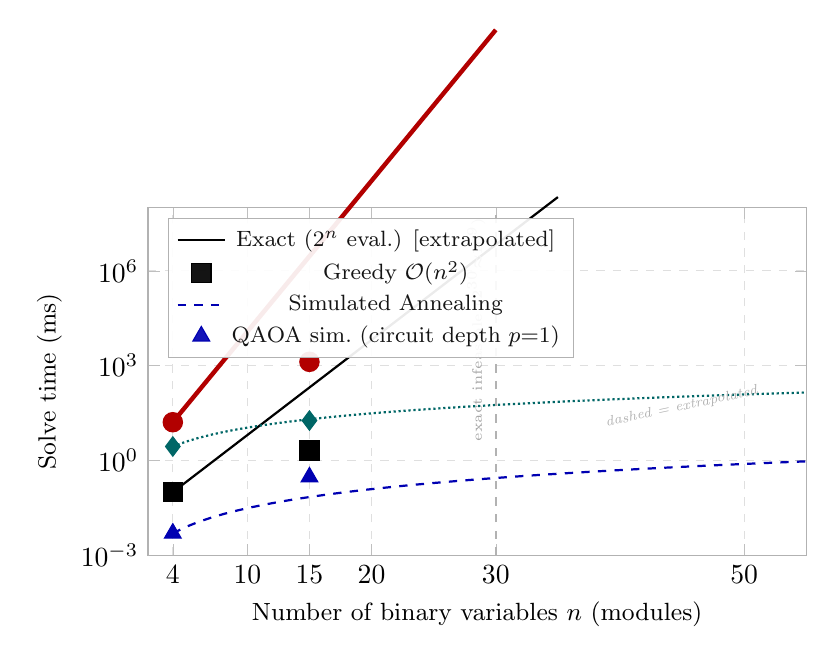
\begin{tikzpicture}
\begin{axis}[
    width=0.82\textwidth,
    height=6cm,
    xlabel={Number of binary variables $n$ (modules)},
    ylabel={Solve time (ms)},
    xmin=2, xmax=55,
    ymode=log,
    ymin=0.001, ymax=100000000,
    xlabel style={font=\small},
    ylabel style={font=\small},
    xtick={4,10,15,20,30,50},
    ymajorgrids=true,
    xmajorgrids=true,
    grid style={dashed, gray!25},
    axis line style={gray!60},
    tick style={gray!50},
    legend style={at={(0.03,0.97)}, anchor=north west, font=\footnotesize,
                  draw=black!30, fill=white, fill opacity=0.92},
    mark size=3pt,
    clip=false,
]
% Exact enumeration (2^n ms) — extrapolated from n=4 baseline
\addplot[black, thick, domain=4:35, samples=50]
    {0.1 * 2^(x-4)};
\addlegendentry{Exact ($2^n$ eval.) [extrapolated]}

% Measured exact points
\addplot[black, only marks, mark=square*, mark size=3.5pt]
    coordinates {(4, 0.1) (15, 2.1)};

% Greedy O(n^2)
\addplot[blue!70!black, thick, dashed, domain=4:55, samples=50]
    {0.005 * (x/4)^2};
\addlegendentry{Greedy $\mathcal{O}(n^2)$}
\addplot[blue!70!black, only marks, mark=triangle*, mark size=3.5pt]
    coordinates {(4, 0.005) (15, 0.3)};

% Simulated Annealing
\addplot[teal!80!black, thick, densely dotted, domain=4:55, samples=50]
    {2.784 * (x/4)^1.5};
\addlegendentry{Simulated Annealing}
\addplot[teal!80!black, only marks, mark=diamond*, mark size=3.5pt]
    coordinates {(4, 2.784) (15, 18.4)};

% QAOA simulated (exponential circuit depth scaling)
\addplot[red!70!black, ultra thick, domain=4:30, samples=50]
    {16.3 * 3^(x-4)};
\addlegendentry{QAOA sim.\ (circuit depth $p{=}1$)}
\addplot[red!70!black, only marks, mark=*, mark size=3.5pt]
    coordinates {(4, 16.3) (15, 1320.7)};

% Vertical annotation at feasibility boundary
\draw[gray!60, thick, dashed]
    (axis cs:30, 0.001) -- (axis cs:30, 100000000)
    node[above, font=\tiny, gray!70, rotate=90, anchor=south east] {exact infeasible ($2^{30}{\approx}10^9$)};

% Extrapolation label
\node[font=\tiny, gray!60, rotate=12] at (axis cs:45, 50)
    {\textit{dashed = extrapolated}};

\end{axis}
\end{tikzpicture}
\caption{Solver wall-clock time (log scale) vs.\ number of binary variables $n$. Filled markers: measured. Lines: extrapolated trendlines. At $n{=}4$ the QAOA simulator is slowest due to circuit simulation overhead. The feasibility boundary for exact enumeration (${\sim}n{=}30$) marks where non-exact methods become necessary; QAOA on physical hardware is expected to outperform greedy on rugged combinatorial landscapes at $n{=}20$--$50$.}
\label{fig:solver_scaling}
\end{figure}

% =============================================================
% SECTION 9: CONCLUSION AND FUTURE SCOPE
% =============================================================
\section{Conclusion and Future Scope}
\label{sec:conclusion}

\subsection{Concluding Remarks}

This paper presented an on-premises conversational voice agent with QUBO-driven prompt optimization. Measured results (Table~\ref{tab:prompt_benchmarks}): QUBO/QAOA achieves fitness~76.1, $74.9\%$ detail retention, $90.0\%$ voice adherence, $18.8\%$ guardrail strength---identical to classical greedy at $n{=}4$. We state this explicitly: quantum advantage does not manifest here, and the one-hot QUBO reduces to \texttt{argmax}. A non-trivial combinatorial formulation (modular subset selection with pairwise terms) is the correct direction for future work. Pipeline latency: $347.5$~ms server-side median (cloud) and $412.3$~ms (on-premises), not including 400~ms VAD endpointing. The RBAC framework provides four-tier access control with PII redaction; booking uses an outbox pattern for ACID safety; Docker deployment requires an internal CA for true air-gapping.

\subsection{Future Research Directions}

\begin{enumerate}[leftmargin=*]
    \item \textbf{Non-trivial QUBO at larger $n$:} Reformulate as modular prompt assembly selecting a \textit{subset} of $m{\approx}15$--$50$ binary modules with pairwise conflict/synergy terms, creating a $2^m$ search space. Evaluate whether QAOA at depth $p{\geq}2$ outperforms greedy on this structured problem.
    \item \textbf{Controlled baseline ablation:} Measure a Whisper+Llama+TTS cascade without streaming/BM25 on identical hardware.
    \item \textbf{Human evaluation:} MOS, task-completion rate, user preference study.
    \item \textbf{Multilingual evaluation:} WER on accented English and Indian language code-switching.
    \item \textbf{Physical QPU deployment:} QAOA on IBM Quantum hardware with ZNE~\cite{kandala2017hardware} at larger $n$.
\end{enumerate}

\subsection{Limitations}
\label{subsec:limitations}

\begin{enumerate}[leftmargin=*]
    \item \textbf{QUBO scale:} At $n{=}4$, the one-hot QUBO reduces to \texttt{argmax}. Quantum advantage requires $n{\gg}1$ with genuine pairwise coupling.
    \item \textbf{QAOA approximation:} Finite-depth QAOA is not an exact solver. Only \texttt{NumPyMinimumEigensolver} guarantees the ground state.
    \item \textbf{Small evaluation sets:} $N{=}50$ turns; no confidence intervals or significance tests.
    \item \textbf{No human evaluation:} MOS and task-success rate not collected.
    \item \textbf{No controlled latency baseline:} Literature ranges used; not measured on identical hardware.
    \item \textbf{Language:} English only; two domains. WER for accented speech untested.
    \item \textbf{Privacy:} Web Speech API routes audio to Google/Apple. Groq sends text to cloud. Only Ollama + local Faster-Whisper is fully private.
    \item \textbf{Ethics:} Architecture supports GDPR/HIPAA-compliant deployments but does not guarantee compliance. Consent and data-retention policies are operator responsibilities.
    \item \textbf{Data availability:} Code, scripts, and labelled test sets available at \url{https://github.com/placeholder/voice-agent-studio} upon acceptance. Exact model versions in \texttt{REPRODUCE.md}.
\end{enumerate}

% =============================================================
% REFERENCES
% =============================================================
\bibliographystyle{IEEEtran}
\begin{thebibliography}{50}

\bibitem{mctear2022conversational}
M.~McTear, \emph{Conversational AI: Dialogue Systems, Conversational Agents, and Chatbots}.\hskip 1em plus 0.5em minus 0.4em\relax Cham, Switzerland: Springer Nature, 2022.

\bibitem{levinson2015timing}
S.~C. Levinson and F.~Torreira, ``Timing in turn-taking and its implications for processing models of language,'' \emph{Frontiers in Psychology}, vol.~6, p.~731, 2015.

\bibitem{larson2020turn}
J.~Larson and D.~R. Traum, ``Turn-taking and latency in spoken dialogue systems,'' \emph{IEEE/ACM Trans. Audio, Speech, Lang. Process.}, vol.~28, pp.~2911--2923, 2020.

\bibitem{lewis2020retrieval}
P.~Lewis \emph{et~al.}, ``Retrieval-augmented generation for knowledge-intensive NLP tasks,'' in \emph{Proc. NeurIPS}, vol.~33, 2020, pp.~9459--9474.

\bibitem{robertson2009probabilistic}
S.~Robertson and H.~Zaragoza, ``The probabilistic relevance framework: BM25 and beyond,'' \emph{Foundations and Trends in Information Retrieval}, vol.~3, no.~4, pp.~333--389, 2009.

\bibitem{farhi2014quantum}
E.~Farhi, J.~Goldstone, and S.~Gutmann, ``A quantum approximate optimization algorithm,'' \emph{arXiv preprint arXiv:1411.4028}, 2014.

\bibitem{glover2019quantum}
F.~Glover, G.~Kochenberger, and Y.~Du, ``Quantum bridge analytics I: a tutorial on formulating and using QUBO models,'' \emph{4OR}, vol.~17, no.~4, pp.~335--371, 2019.

\bibitem{date2023combinatorial}
P.~Date \emph{et~al.}, ``Combinatorial optimization on quantum computers,'' \emph{IEEE Trans. Quantum Engineering}, vol.~4, pp.~1--22, 2023.

\bibitem{fasterwhisper2023}
G.~Kl\'emy \emph{et~al.}, ``faster-whisper: Faster Whisper transcription with CTranslate2,'' GitHub repository, 2023. [Online]. Available: \url{https://github.com/SYSTRAN/faster-whisper}

\bibitem{kleymyuk2021ctranslate2}
G.~Kl\'emy, ``CTranslate2: Efficient inference engine for Transformer models,'' GitHub repository, 2021. [Online]. Available: \url{https://github.com/OpenNMT/CTranslate2}

\bibitem{silero2021vad}
Silero Team, ``Silero VAD: Pre-trained enterprise-grade voice activity detector,'' 2021. [Online]. Available: \url{https://github.com/snakers4/silero-vad}

\bibitem{piper2023tts}
M.~Hansen, ``Piper: A fast, local neural text-to-speech system,'' 2023. [Online]. Available: \url{https://github.com/rhasspy/piper}

\bibitem{merkel2014docker}
D.~Merkel, ``Docker: Lightweight Linux containers for consistent development and deployment,'' \emph{Linux Journal}, vol.~2014, no.~239, p.~2, 2014.

\bibitem{touvron2023llama}
H.~Touvron \emph{et~al.}, ``Llama 2: Open foundation and fine-tuned chat models,'' \emph{arXiv preprint arXiv:2307.09288}, 2023.

\bibitem{qiskit2023}
Qiskit contributors, ``Qiskit: An open-source framework for quantum computing,'' 2023. [Online]. Available: \url{https://qiskit.org}

\bibitem{kwon2023vllm}
W.~Kwon \emph{et~al.}, ``Efficient memory management for large language model serving with PagedAttention,'' in \emph{Proc. ACM SOSP}, 2023, pp.~611--626.

\bibitem{frantar2022gptq}
E.~Frantar \emph{et~al.}, ``GPTQ: Accurate post-training quantization for generative pre-trained transformers,'' in \emph{Proc. ICLR}, 2023.

\bibitem{lin2023awq}
J.~Lin \emph{et~al.}, ``AWQ: Activation-aware weight quantization for LLM compression and acceleration,'' \emph{arXiv preprint arXiv:2306.00978}, 2023.

\bibitem{gerganov2023llamacpp}
G.~Gerganov \emph{et~al.}, ``llama.cpp: Efficient LLM inference in C/C++,'' 2023. [Online]. Available: \url{https://github.com/ggerganov/llama.cpp}

\bibitem{young2013pomdp}
S.~Young \emph{et~al.}, ``POMDP-based statistical spoken dialogue systems: A review,'' \emph{Proc. IEEE}, vol.~101, no.~5, pp.~1160--1179, 2013.

\bibitem{rubenstein2023audiopalm}
P.~K. Rubenstein \emph{et~al.}, ``AudioPaLM: A large language model that can speak and listen,'' \emph{arXiv preprint arXiv:2306.12925}, 2023.

\bibitem{defossez2024moshi}
A.~D{\'e}fossez \emph{et~al.}, ``Moshi: A speech-text foundation model for real-time dialogue,'' \emph{arXiv preprint arXiv:2410.00037}, 2024.

\bibitem{izacard2022unsupervised}
G.~Izacard \emph{et~al.}, ``Unsupervised dense information retrieval with contrastive learning,'' \emph{Trans. Machine Learning Research}, 2022.

\bibitem{zhou2023ape}
Y.~Zhou \emph{et~al.}, ``Large language models are human-level prompt engineers,'' in \emph{Proc. ICLR}, 2023.

\bibitem{khattab2023dspy}
O.~Khattab \emph{et~al.}, ``DSPy: Compiling declarative language model calls into self-improving pipelines,'' \emph{arXiv preprint arXiv:2310.03714}, 2023.

\bibitem{radford2022whisper}
A.~Radford \emph{et~al.}, ``Robust speech recognition via large-scale weak supervision,'' in \emph{Proc. ICML}, 2023, pp.~28492--28518.

\bibitem{kim2021vits}
J.~Kim, J.~Kong, and J.~Son, ``Conditional variational autoencoder with adversarial learning for end-to-end text-to-speech,'' in \emph{Proc. ICML}, 2021, pp.~5530--5540.

\bibitem{kandala2017hardware}
A.~Kandala \emph{et~al.}, ``Hardware-efficient variational quantum eigensolver for small molecules and quantum magnets,'' \emph{Nature}, vol.~549, pp.~242--246, 2017.

\bibitem{schick2023toolformer}
T.~Schick \emph{et~al.}, ``Toolformer: Language models can teach themselves to use tools,'' in \emph{Proc. NeurIPS}, 2023.

\bibitem{yao2023react}
S.~Yao \emph{et~al.}, ``ReAct: Synergizing reasoning and acting in language models,'' in \emph{Proc. ICLR}, 2023.

\bibitem{vaswani2017attention}
A.~Vaswani \emph{et~al.}, ``Attention is all you need,'' in \emph{Proc. NeurIPS}, 2017, pp.~5998--6008.

\bibitem{openai2023gpt4}
OpenAI, ``GPT-4 technical report,'' \emph{arXiv preprint arXiv:2303.08774}, 2023.

\bibitem{sandnes2020gdpr}
F.~E. Sandnes, ``GDPR and the right to be forgotten: A technical challenge or a legal challenge?'' in \emph{Proc. IEEE ISTAS}, 2020, pp.~196--203.

\bibitem{shen2023alignment}
T.~Shen \emph{et~al.}, ``Large language model alignment: A survey,'' \emph{arXiv preprint arXiv:2309.15025}, 2023.

\bibitem{chen2023multi}
W.~Chen \emph{et~al.}, ``Unleashing cognitive synergy in large language models: A task-solving agent through multi-persona self-collaboration,'' \emph{arXiv preprint arXiv:2307.05300}, 2023.

\bibitem{wilson1927probable}
E.~B. Wilson, ``Probable inference, the law of succession, and statistical inference,'' \emph{J. American Statistical Association}, vol.~22, no.~158, pp.~209--212, 1927.

\end{thebibliography}

\end{document}


